\PassOptionsToPackage{unicode=true}{hyperref} % options for packages loaded elsewhere
\PassOptionsToPackage{hyphens}{url}
%
\documentclass[]{article}
\usepackage{lmodern}
\usepackage{amssymb,amsmath}
\usepackage{ifxetex,ifluatex}
\usepackage{fixltx2e} % provides \textsubscript
\ifnum 0\ifxetex 1\fi\ifluatex 1\fi=0 % if pdftex
  \usepackage[T1]{fontenc}
  \usepackage[utf8]{inputenc}
  \usepackage{textcomp} % provides euro and other symbols
\else % if luatex or xelatex
  \usepackage{unicode-math}
  \defaultfontfeatures{Ligatures=TeX,Scale=MatchLowercase}
\fi
% use upquote if available, for straight quotes in verbatim environments
\IfFileExists{upquote.sty}{\usepackage{upquote}}{}
% use microtype if available
\IfFileExists{microtype.sty}{%
\usepackage[]{microtype}
\UseMicrotypeSet[protrusion]{basicmath} % disable protrusion for tt fonts
}{}
\IfFileExists{parskip.sty}{%
\usepackage{parskip}
}{% else
\setlength{\parindent}{0pt}
\setlength{\parskip}{6pt plus 2pt minus 1pt}
}
\usepackage{hyperref}
\hypersetup{
            pdftitle={A Course on Price Indices},
            pdfauthor={Steve Martin},
            pdfborder={0 0 0},
            breaklinks=true}
\urlstyle{same}  % don't use monospace font for urls
\usepackage[margin=1in]{geometry}
\usepackage{color}
\usepackage{fancyvrb}
\newcommand{\VerbBar}{|}
\newcommand{\VERB}{\Verb[commandchars=\\\{\}]}
\DefineVerbatimEnvironment{Highlighting}{Verbatim}{commandchars=\\\{\}}
% Add ',fontsize=\small' for more characters per line
\usepackage{framed}
\definecolor{shadecolor}{RGB}{248,248,248}
\newenvironment{Shaded}{\begin{snugshade}}{\end{snugshade}}
\newcommand{\AlertTok}[1]{\textcolor[rgb]{0.94,0.16,0.16}{#1}}
\newcommand{\AnnotationTok}[1]{\textcolor[rgb]{0.56,0.35,0.01}{\textbf{\textit{#1}}}}
\newcommand{\AttributeTok}[1]{\textcolor[rgb]{0.77,0.63,0.00}{#1}}
\newcommand{\BaseNTok}[1]{\textcolor[rgb]{0.00,0.00,0.81}{#1}}
\newcommand{\BuiltInTok}[1]{#1}
\newcommand{\CharTok}[1]{\textcolor[rgb]{0.31,0.60,0.02}{#1}}
\newcommand{\CommentTok}[1]{\textcolor[rgb]{0.56,0.35,0.01}{\textit{#1}}}
\newcommand{\CommentVarTok}[1]{\textcolor[rgb]{0.56,0.35,0.01}{\textbf{\textit{#1}}}}
\newcommand{\ConstantTok}[1]{\textcolor[rgb]{0.00,0.00,0.00}{#1}}
\newcommand{\ControlFlowTok}[1]{\textcolor[rgb]{0.13,0.29,0.53}{\textbf{#1}}}
\newcommand{\DataTypeTok}[1]{\textcolor[rgb]{0.13,0.29,0.53}{#1}}
\newcommand{\DecValTok}[1]{\textcolor[rgb]{0.00,0.00,0.81}{#1}}
\newcommand{\DocumentationTok}[1]{\textcolor[rgb]{0.56,0.35,0.01}{\textbf{\textit{#1}}}}
\newcommand{\ErrorTok}[1]{\textcolor[rgb]{0.64,0.00,0.00}{\textbf{#1}}}
\newcommand{\ExtensionTok}[1]{#1}
\newcommand{\FloatTok}[1]{\textcolor[rgb]{0.00,0.00,0.81}{#1}}
\newcommand{\FunctionTok}[1]{\textcolor[rgb]{0.00,0.00,0.00}{#1}}
\newcommand{\ImportTok}[1]{#1}
\newcommand{\InformationTok}[1]{\textcolor[rgb]{0.56,0.35,0.01}{\textbf{\textit{#1}}}}
\newcommand{\KeywordTok}[1]{\textcolor[rgb]{0.13,0.29,0.53}{\textbf{#1}}}
\newcommand{\NormalTok}[1]{#1}
\newcommand{\OperatorTok}[1]{\textcolor[rgb]{0.81,0.36,0.00}{\textbf{#1}}}
\newcommand{\OtherTok}[1]{\textcolor[rgb]{0.56,0.35,0.01}{#1}}
\newcommand{\PreprocessorTok}[1]{\textcolor[rgb]{0.56,0.35,0.01}{\textit{#1}}}
\newcommand{\RegionMarkerTok}[1]{#1}
\newcommand{\SpecialCharTok}[1]{\textcolor[rgb]{0.00,0.00,0.00}{#1}}
\newcommand{\SpecialStringTok}[1]{\textcolor[rgb]{0.31,0.60,0.02}{#1}}
\newcommand{\StringTok}[1]{\textcolor[rgb]{0.31,0.60,0.02}{#1}}
\newcommand{\VariableTok}[1]{\textcolor[rgb]{0.00,0.00,0.00}{#1}}
\newcommand{\VerbatimStringTok}[1]{\textcolor[rgb]{0.31,0.60,0.02}{#1}}
\newcommand{\WarningTok}[1]{\textcolor[rgb]{0.56,0.35,0.01}{\textbf{\textit{#1}}}}
\usepackage{longtable,booktabs}
% Fix footnotes in tables (requires footnote package)
\IfFileExists{footnote.sty}{\usepackage{footnote}\makesavenoteenv{longtable}}{}
\usepackage{graphicx,grffile}
\makeatletter
\def\maxwidth{\ifdim\Gin@nat@width>\linewidth\linewidth\else\Gin@nat@width\fi}
\def\maxheight{\ifdim\Gin@nat@height>\textheight\textheight\else\Gin@nat@height\fi}
\makeatother
% Scale images if necessary, so that they will not overflow the page
% margins by default, and it is still possible to overwrite the defaults
% using explicit options in \includegraphics[width, height, ...]{}
\setkeys{Gin}{width=\maxwidth,height=\maxheight,keepaspectratio}
\setlength{\emergencystretch}{3em}  % prevent overfull lines
\providecommand{\tightlist}{%
  \setlength{\itemsep}{0pt}\setlength{\parskip}{0pt}}
\setcounter{secnumdepth}{5}
% Redefines (sub)paragraphs to behave more like sections
\ifx\paragraph\undefined\else
\let\oldparagraph\paragraph
\renewcommand{\paragraph}[1]{\oldparagraph{#1}\mbox{}}
\fi
\ifx\subparagraph\undefined\else
\let\oldsubparagraph\subparagraph
\renewcommand{\subparagraph}[1]{\oldsubparagraph{#1}\mbox{}}
\fi

% set default figure placement to htbp
\makeatletter
\def\fps@figure{htbp}
\makeatother


\title{A Course on Price Indices}
\author{Steve Martin}
\date{May 2020}

\begin{document}
\maketitle

{
\setcounter{tocdepth}{2}
\tableofcontents
}
\hypertarget{overview}{%
\section*{Overview}\label{overview}}
\addcontentsline{toc}{section}{Overview}

This course gives a modern and straightforward introduction to prices indices. The focus in on the main ideas and concepts that are important for both users and compilers of price indices; consequently, the course is not encyclopedic, and several important topics are either given a quick treatment, or not covered at all. Many references are provided to complement the material in this course, and extend the scope of the topics covered.

Overall the course rests firmly in the area of theory, and is designed to help foster an understanding of what a price index is. Several practical examples using the R programming language are given throughout the course, along with several applied exercises. But most of the more ``real world'' aspects of making a price index are ignored. This is not because these things are not important; rather, it is difficult to appreciate these more practical topics without a firm grasp of the theory.

The course is broken into four modules that building on each other. The first module gives an introduction to price indices, focusing mainly on the computation aspects of a price index. The second module gives a broad introduction to the theory of price indices, with a focus on motivating the price indices that get produced by national statistical agencies. The third module covers quality adjustments, one of the main practical hurdles when building a price index. The fourth modules brings everything together with an extended exercise to build and analyze a price index with R.

\hypertarget{part-introduction-to-price-indices}{%
\part{Introduction to Price Indices}\label{part-introduction-to-price-indices}}

\hypertarget{syllabus}{%
\section{Syllabus}\label{syllabus}}

A price index gives a way to systematically condense information about many prices for a range of goods and services into a single value. Price indices are widely used to analyze and compare macroeconomic conditions over time, and have important implications for government policies.

The goal of this module is to provide an introduction to price indices, with an application to price indices for the inputs and outputs of production (producer price index), and for prices faced by consumers (consumer price index). By the end of the module, an individual should:

\begin{enumerate}
\def\labelenumi{\arabic{enumi}.}
\item
  Understand the reasons why price indices are compiled, and why they're important.
\item
  Be familiar with common index-number formulas and how to manipulate them.
\item
  Have a basic understanding of the structure of a price index and its calculation.
\end{enumerate}

This module is useful for both users and compilers of price indices with little prior knowledge of the uses and construction of a price index.

This module consists of self-directed readings, along with an assignment. In total, about 10 to 15 hours should be devoted for this module

There are no prerequisites for this module, although individuals should be comfortable with basic algebra and simple mathematical arguments. An introductory course in macroeconomics is helpful.

Evaluation for this module is based on an assignment consisting of 20 multiple-choice/true-false questions that draw on material in the course content and readings. Collaboration on the assignment is welcomed, but each person must submit their own unique work. Passing this module requires at least a 65\% on the assignment.

Readings for this module come from chapters 1, 2, 4, and 9 of the Producer Price Index Manual (ILO et al. 2004b) and/or the Consumer Price Index Manual (ILO et al. 2004a), published by the IMF (freely available on their website). As there is a considerable amount of overlap between these sources, the PPI manual is used as the main reference.

Please email the course instructor if you have any questions, or need help with any of the course material or assignment.

\hypertarget{whats-a-price-index-and-why-do-we-need-one}{%
\section{What's a price index and why do we need one?}\label{whats-a-price-index-and-why-do-we-need-one}}

A price index is a tool to measure the change in price for goods and services over time. Price indices have a long history, and are an important and widely used macroeconomic statistic. This section of the course begins by introducing what a price index is, what they're used for, and why a price index is needed at all.

📖 PPI manual: Chapter 1, sections A, K; Chapter 2, sections A, B, D1, D2, E, F.

📖 CPI manual: Chapter 1, paragraphs 1.8--1.12; Chapter 2.

\hypertarget{whats-a-price-index}{%
\subsection{What's a price index?}\label{whats-a-price-index}}

A price index is an economic time series that gives the percent change in prices for a collection of goods and services between a given point in time and a fixed reference point in time (i.e., the base period or reference period).\footnote{A price index can also be used to measure the difference in prices in different locations at the same point in time, although this is a less common use of a price index.} A price index is usually represented so that subtracting 100 from the value of the index gives the percent change in prices for the goods and services captured by the index. For example, if a price index for widgets has a value of 110 in some period, then prices for widgets have increased by 10\% since the base period. This representation also means that the index has a value of 100 in the base period.

The chart below gives an example of a monthly price index showing the change in prices in each month of the year with respect to January (the base period), so that each point on the graph gives the percent change in prices since January. For example, in March the index had a value of 103, meaning prices increased by 3\% between March and January, whereas the index had a value of 99 in June, meaning prices decreased by 1\% between January and June.

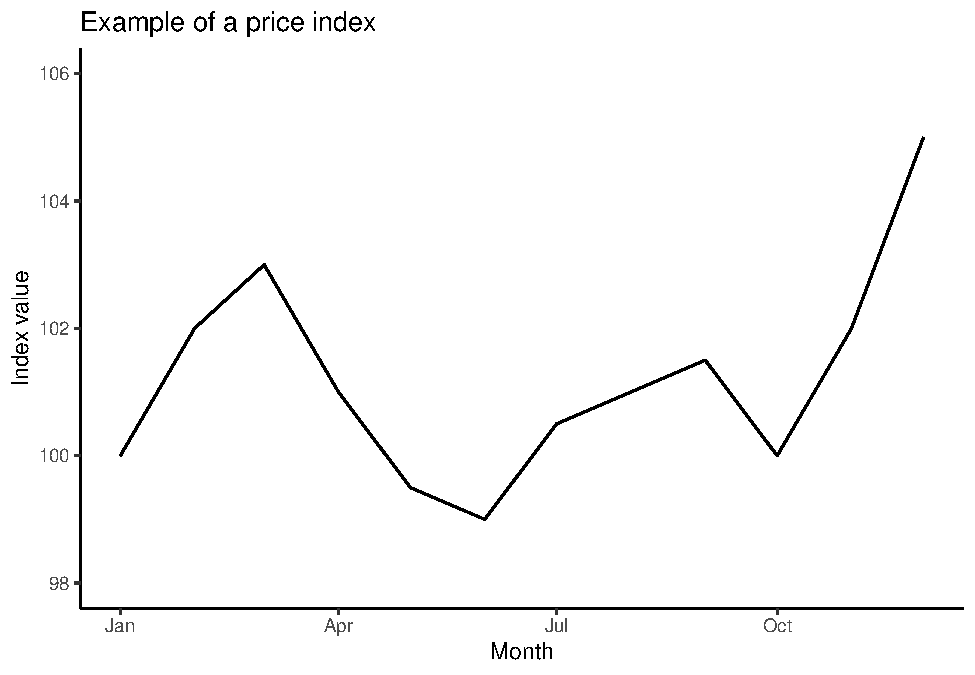
\includegraphics{price-index-course_files/figure-latex/unnamed-chunk-1-1.pdf}

Since a price index only measures the relative change in prices since the base period, changing the scale of the index does not change its economic content. For example, dividing all values in the above chart by 100 does not change the shape of the graph, or the resulting percent change in the index value since the base period. It is for this reason that the magnitude of a price index does not give a measure of the price level at a point in time---a price index can only measure the change in prices over time.

The usefulness of a price index is that it gives a way to systematically condense information about many prices for a range of goods and services into a single value that measures the change in prices for these goods and services over time. Although which goods and services form the scope of a price index depends on its purpose, all price indices give a measure of aggregate price movements for a well-defined set of commodities. This in turn gives a measure of inflationary pressures in an economy, and consequently price indices are ubiquitous when examining macroeconomic conditions and policies.

\hypertarget{uses-of-a-price-index}{%
\subsection{Uses of a price index}\label{uses-of-a-price-index}}

In practice there are two broad categories that the price indices published by national statistical agencies fall into: consumer price indices (CPIs) and producer price indices (PPIs). As the names suggest, CPIs are focused on measuring price changes for goods and services that are purchased by consumers (final consumption), whereas PPIs focus on measuring prices charged by producers for goods and services produced, and prices paid for inputs into production. Despite the many subtleties about what constitutes a consumer and what constitutes a producer, both CPIs and PPIs seek to measure the change in prices over time for the goods and services that are transacted in an economy. Consequently, there is often
considerable overlap in how CPIs and PPIs are calculated and used, and a distinction does not need to be made between whether an index is a CPI or a PPI---it often suffices to talk about a general price index.

Probably the most important use of a price index, be it a CPI or a PPI, is to measure inflation---the systematic change in prices in an economy over time. Beyond being an important macroeconomic indicator, the measure of inflation directly affects many economic interactions in modern economies. For instance, many central banks operate in a regime of inflation targeting, whereby monetary policy is conducted in part to keep the inflation rate in a predetermined range (e.g., 1\% to 3\% a year). This policy regime requires a frequent and timely measure of inflation, and the instrument used to measure inflation can have a direct impact on monetary policy, and consequently interest rates. Inflation also affects wages and service contracts, pension payments, and social security benefits, as these contracts are often indexed to inflation---if prices increase by 2\% per year, then wages also increase by 2\% per year. Indexation preserves the value of payments over time without constantly needing to renegotiate contracts or redesign policies. The measure of inflation thus has important implications for household income and industry revenues.

Beyond measuring inflation, one of the major uses of price indices for national statistical agencies is to deflate aggregate values in a national accounting framework to get a measure of the change in the production of real goods and services over time. This is equivalent to finding a quantity index to systematically condense information about many outputs for a range of goods and services into a single value that measures the change in the quantity of goods and services produced over time. Although there are many details, the rationale behind deflating aggregate values to get a measure of real output is fairly simple. If \(V_1/V_0\) is the ratio of the value of production in period 1 to the value of production in period 0, and if this can be decomposed into a quantity index \(Q\) and a price index \(I\) such that \(V_1/V_0 = IQ\), then the change in real production between period 0 and period 1 is simply \(Q = V_1 / (V_0 I)\). The change in the value of production over time---a known quantity---can be turned into a measure of the change in real output by simply deflating it with a price index.

\hypertarget{why-a-price-index}{%
\subsection{Why a price index?}\label{why-a-price-index}}

The starting point for understanding the utility of a price index is recognizing that there is no need for one if the goal is to compare the price of a single good or service in one period to the price for the same good or service in another period. If \(p_1\) is the price of a good in period 1 and \(p_0\) is the price of that same good in period 0, then the price relative \(p_1/p_0\) unambiguously gives the percent change in price between period 1 and period 0. The need for a price index arises out of a fundamental problem of comparing a collection of two or more prices at two points in time to arrive at an overall change in price.

To illustrate this comparison problem, suppose there are two goods, denoted by \(i\) and \(j\), that sell in periods 0 and 1. If the price of good \(i\) and the price of good \(j\) both increase between period 0 and period 1, then it is uncontroversial to say that prices have increased between period 0 and period 1 (although it is less obvious by how much prices have increased). Similarly, if both prices decrease, then it is natural to say that prices have decreased. However, an issue arises if the price of good \(i\) increases between period 0 and
period 1 while the price of good \(j\) decreases. In this case it is unclear if prices have increased or decreased---there is no obvious way to give a single direction to the movement of prices over time.

A solution to this comparison problem is to find a way to aggregate price relatives for many goods and services together to form a single ratio, which is then interpreted as the overall movement in prices over time. This is the job of a price index. Although a price index solves the comparison problem, it introduces a new challenge---how to best combine price relatives to produce a single measure that describes overall change in prices. Consequently, a variety of index-number formulas have been proposed to construct a price index.

\hypertarget{index-number-formula}{%
\section{Index-number formula}\label{index-number-formula}}

There are a great many index-number formula that can be used to combine information on prices at two points in time to produce a price index, despite the common goal of measuring price changes over time. This section of the course covers 10 important index-number formulas that are used in practice to calculate a price index. Associated with each formula is the name of the person who developed it. It is important to associate the names with the formulas, as they are usually referred to by name in application. This is unfortunately an exercise is memorization, as most of the index-number formula have a similar form.

To help build intuition and a deeper understanding of what the index-number formula are doing, these different approaches for calculating a price index can be broadly classified as either arithmetic price indices or geometric price indices. Not all index-number formula fall into these two groups---for example, there are also harmonic price indices, a category which can overlap with arithmetic indices---but arithmetic and geometric indices are fairly easy to understand, with most index-number formulas falling into one of these two categories.

In practice a price index is multiplied by 100, so that the percent change in the index value over two periods is simply the index value minus 100. This is just a convenient normalization that has no bearing on the economic content of a price index, and is ignored in this section. Note that all the index-number formulas can be multiplied by 100 to put them on the usual scale.

📖 PPI manual: Chapter 1, sections B1--B3.

\hypertarget{arithmetic-price-indices}{%
\subsection{Arithmetic price indices}\label{arithmetic-price-indices}}

An arithmetic price index takes price relatives for a collection of goods and services over two periods and combines them together as a weighted average. That is, an arithmetic index is simply the average change in price between two points in time. Letting goods be enumerated by \(i = 1,\ldots, n\), an arithmetic index between period 0 and period 1 has the general form\footnote{The capital letter sigma \(\Sigma\) is the summation operator. For a collection of numbers \(x_{1}, x_{2},\ldots,x_{n}\), \(\sum_{i=1}^{n} x_{i}\) means \(x_{1} + x_{2} + \ldots + x_{n}\).}

\begin{align*}
I^{A} = \sum_{i = 1}^{n} \omega_{i} \frac{p_{i1}}{p_{i0}},
\end{align*}

where \(p_{it}\) is the price of good \(i\) in period \(t = 0,1\), and \(\omega_{i} \geq 0\) is the weight that good \(i\) receives in the index calculation, such that \(\sum_{i = 1}^{n} \omega_{i} = 1\).

Different arithmetic price indices correspond to special cases of the general arithmetic index, depending on the choice of the weights. Most of these choices make use of information about the quantity of a good sold, so that the weights give a measure of the economic importance of a good. Denote by \(q_{it}\) the amount of good \(i\) consumed/produced in period \(t = 0,1\).

Before examining specific arithmetic indices, it is worth noting that an arithmetic index can always be written as the ratio of expenditure/revenue for a ``basket'' of goods and services at two points in time, so that for any set of weights there are implied ``quantities'' such that

\begin{align*}
I^{A} = \frac{\sum_{i = 1}^{n} p_{i1} \tilde{q}_{i}}{\sum_{i = 1}^{n} p_{i0} \tilde{q}_{i}},
\end{align*}

where \(\tilde{q}_{i} = \alpha \omega_{i} / p_{i0}\) for some factor of proportionality \(\alpha\).\footnote{The value of \(\alpha\) has no impact on the index, but is needed to property interpret \(\tilde{q}_{i}\) as a quantity. For example, if \(\omega_{i}\) is the period-0 expenditure share on good \(i\), \(p_{i0} q_{i0} / \sum_{j = 1}^{n} p_{j0} q_{j0}\), then \(\alpha = \sum_{j = 1}^{n} p_{j0} q_{j0}\) so that \(\tilde{q}_{i} = q_{i0}\).} Thus, an arithmetic index can always be interpreted as the ratio of the expenditure required to purchase a fixed basket of goods at two points in time (or the revenue from a fixed basket of goods at two points in time). The choice of basket is linked one-to-one with the choice of weights used to aggregate price relatives. Both representations of the arithmetic index get used, as some indices are easier to represent in one form than the other.

\hypertarget{common-arithmetic-indices}{%
\subsection{Common arithmetic indices}\label{common-arithmetic-indices}}

There are six main arithmetic price indices that get used in practice, each corresponding to a different statement about how much weight a price relative should receive in the index calculation.

\textbf{Carli index}. Setting \(\omega_{i} = 1 / n\) results in the Carli index

\begin{align*}
I^{A}_{C} = \frac{1}{n} \sum_{i = 1}^{n} \frac{p_{i1}}{p_{i0}}.
\end{align*}

The Carli index takes a neutral stance on the weights, and treats each price relative as equally important.

\textbf{Dutot index}. Setting \(\omega_{i} = p_{i0} / \sum_{j = 1}^{n} p_{j0}\) results in the Dutot index

\begin{align*}
I^{A}_D = \frac{\sum_{i = 1}^{n} p_{i1}}{\sum_{i = 1}^{n} p_{i0}}.
\end{align*}

The Dutot index gives more weight to price relatives that have a greater period-0 price, comparing the average price of goods in period 1 to the average price in period 0.

\textbf{Lowe index}. Setting \(\omega_{i} = p_{i0} q_{ib} / \sum_{j = 1}^{n} p_{j0} q_{jb}\) results in the Lowe index

\begin{align*}
I^{A}_{l} = \frac{\sum_{i = 1}^{n} p_{i1} q_{ib}}{\sum_{i = 1}^{n} p_{i0} q_{ib}},
\end{align*}

where \(q_{ib}\) is the quantity of good \(i\) in some base period \(b\), usually prior to period 0. The weights for the Lowe index are ``hybrid'' expenditure/revenue shares for the basket of goods and services in period \(b\) using period 0 prices.

\textbf{Laspeyres index}. Setting \(\omega_{i} = p_{i0} q_{i0} / \sum_{j = 1}^{n} p_{j0} q_{j0}\) results in the Laspeyres index

\begin{align*}
I^{A}_{L} = \frac{\sum_{i = 1}^{n} p_{i1} q_{i0}}{\sum_{i = 1}^{n} p_{i0} q_{i0}}.
\end{align*}

The Laspeyres index weights price relatives according to their period-0 expenditure/revenue share, and is a special case of the Lowe index.

\textbf{Paasche index}. Setting \(\omega_{i} = p_{i0} q_{i1} / \sum_{j = 1}^{n} p_{j0} q_{j1}\) results in the Paasche index

\begin{align*}
I^{A}_{P} = \frac{\sum_{i = 1}^{n} p_{i1} q_{i1}}{\sum_{i = 1}^{n} p_{i0} q_{i1}}.
\end{align*}

Like the Laspeyres index, the Paasche index is a special case of the Lowe index, and uses hybrid expenditure/revenue shares to weight price relatives.

It is worth noting that the Paasche index is often calculated as a weighted harmonic average, with period 1 expenditure/revenue shares as weights, so that

\begin{align*}
I^{A}_{P} = \left(\sum_{i = 1}^{n} \frac{\frac{p_{i1} q_{i1}}{\sum_{j = 1}^{n} p_{j1} q_{j1}}}{\frac{p_{i1}}{p_{i0}}}\right)^{-1}.
\end{align*}

This is an example of a harmonic price index, and is a convenient way to calculate a Paasche index if only period-1 expenditure/revenue shares are known, rather than period-1 quantities.

\textbf{Young index}. Setting \(\omega_{i} = p_{ib} q_{ib} / \sum_{j = 1}^{n} p_{jb} q_{jb}\) results in the Young index

\begin{align*}
I^{A}_{Y} = \sum_{i = 1}^{n} \frac{p_{ib} q_{ib}}{\sum_{j = 1}^{n} p_{jb} q_{jb}} \frac{p_{i1}}{p_{i0}},
\end{align*}

where \(q_{ib}\) is the quantity of good \(i\) in some base period \(b\), with \(p_{ib}\) as the price, usually prior to period 0. The Young index uses period \(b\) expenditure/revenue shares as weights.\footnote{In some cases a Young index is used to refer to a general arithmetic index, rather than an arithmetic index with a particular set of weights.} The Laspeyres index is a special case of the Young index.

In most applications a Laspeyres index is the desired index-number formula for an arithmetic price index, in part because the weights can be observed separately from the price information. Weights for a CPI, for example, can come from a nationally representative survey of household spending, and so only price information needs to be collected to calculate a Laspeyres index. Although the Young weights are directly observable as well, they do not necessarily reflect changes in the composition of spending or sources of revenue between period \(b\) and period 0. Alternatively, both the Lowe and Paasche indices have weights that need to be explicitly calculated. Like the Young index, the Lowe index uses out-of-date quantity information, whereas the Paasche index uses current-period quantity information, and this usually means that it cannot be computed in a timely manner.

Despite the goal of calculating a Laspeyres index, in most applications an arithmetic index is often calculated as a Young index (or sometimes a Lowe index), as it is difficult to get timely expenditure/revenue share information. Waiting for the weighting information may require delaying the production of an index until well after period 0. The hope is that the weights used in the Young index offer a reasonable approximation for the Laspeyres weights.

\hypertarget{less-common-arithmetic-indices}{%
\subsection{Less common arithmetic indices}\label{less-common-arithmetic-indices}}

There are a variety of arithmetic indices that are rarely used in practice, but can be useful to know about. As these index-number formulas are seldom used, this material can be safely be skipped.

\textbf{Palgrave index}. Setting \(\omega_{i} = p_{i1} q_{i1} / \sum_{j = 1}^{n} p_{j1} q_{j1}\) results in the Palgrave index

\begin{align*}
I^{A}_{p} = \sum_{i = 1}^{n} \frac{p_{i1} q_{i1}}{\sum_{j = 1}^{n} p_{j1} q_{j1}} \frac{p_{i1}}{p_{i0}}.
\end{align*}

The Palgrave index uses period-1 expenditure shares as weights, and is a special case of the Young index.

\textbf{Unnamed index}. Setting

\begin{align*}
\omega_{i} = \frac{1}{2} \frac{p_{i0} q_{i0}}{\sum_{j = 1}^{n} p_{j0} q_{j0}} + \frac{1}{2} \frac{p_{i1} q_{i1}}{\sum_{j = 1}^{n} p_{j1} q_{j1}}
\end{align*}

results in an index-number formula without a name,

\begin{align*}
I^{A}_{U} = \sum_{i = 1}^{n} \left(\frac{1}{2} \frac{p_{i0} q_{i0}}{\sum_{j = 1}^{n} p_{j0} q_{j0}} + \frac{1}{2} \frac{p_{i1} q_{i1}}{\sum_{j = 1}^{n} p_{j1} q_{j1}}\right) \frac{p_{i1}}{p_{i0}}.
\end{align*}

This index is a mixture of the Laspeyres and Palgrave indices, with weights given by the average expenditure/revenue share between period 0 and period 1.

\textbf{Drobisch index}. Setting

\begin{align*}
\omega_{i} = \frac{1}{2} \frac{p_{i0} q_{i0}}{\sum_{j = 1}^{n} p_{j0} q_{j0}} + \frac{1}{2} \frac{p_{i0} q_{i1}}{\sum_{j = 1}^{n} p_{j0} q_{j1}}
\end{align*}

results in the Drobisch index

\begin{align*}
I^{A}_{d} = \frac{1}{2} \frac{\sum_{i = 1}^{n} p_{i1} q_{i0}}{\sum_{i = 1}^{n} p_{i0} q_{i0}} + \frac{1}{2} \frac{\sum_{i = 1}^{n} p_{i1} q_{i1}}{\sum_{i = 1}^{n} p_{i0} q_{i1}}.
\end{align*}

This index is a mixture of the Laspeyres and Paasche indices.

\textbf{Walsh index}. Setting \(\omega_{i} = p_{i0} \sqrt{q_{i0} q_{i1}} / \sum_{j = 1}^{n} p_{j0} \sqrt{q_{j0} q_{j1}}\) results in the Walsh index

\begin{align*}
I^{A}_{W} = \frac{\sum_{i = 1}^{n} p_{i1} \sqrt{q_{i0} q_{i1}}}{\sum_{i = 1}^{n} p_{i0} \sqrt{q_{i0} q_{i1}}}.
\end{align*}

This index uses a basket that contains the geometric average of the period-0 and period-1 quantities.

\textbf{Marshall-Edgeworth index}. Setting \(\omega_{i} = p_{i0} (q_{i0} + q_{i1}) / \sum_{j = 1}^{n} p_{j0} (q_{j0} + q_{j1})\) results in the Marshall-Edgeworth index

\begin{align*}
I^{A}_{M} = \frac{\sum_{i = 1}^{n} p_{i1} (q_{i0} + q_{i1}) / 2}{\sum_{i = 1}^{n} p_{i0} (q_{i0} + q_{i1}) / 2}.
\end{align*}

Like the Walsh index, this index uses a basket that takes an average of the period-0 and period-1 quantities.

\textbf{Geary-Khamis index}. Setting \(\omega_{i} = p_{i0} / (1 / q_{i0} + 1 / q_{i1}) / \sum_{j = 1}^{n} p_{j0} / (1 / q_{j0} + 1 / q_{j1})\) results in the Geary-Khamis index

\begin{align*}
I^{A}_{G} = \frac{\sum_{i = 1}^{n} 2 p_{i1} / (1 / q_{i0} + 1 / q_{i1})}{\sum_{i = 1}^{n} 2 p_{i0} / (1 / q_{i0} + 1 / q_{i1})}.
\end{align*}

Like the Walsh and Marshall-Edgeworth indices, this index uses a basket that takes an average of the period-0 and period-1 quantities.

\hypertarget{geometric-price-indices}{%
\subsection{Geometric price indices}\label{geometric-price-indices}}

A geometric price index is entirely analogous to an arithmetic one, except that price relatives are aggregated with a geometric average instead of an arithmetic average. That is, a general geometric price index is given by\footnote{The capital letter pi \(\Pi\) is the product operator. For a collection of numbers \(x_{1}, x_{2},\ldots,x_{n}\), \(\prod_{i=1}^{n} x_{i}\) means \(x_{1} \times x_{2} \times \ldots \times x_{n}\).}

\begin{align*}
I^{G} = \prod_{i = 1}^{n} \left(\frac{p_{i1}}{p_{i0}}\right)^{\omega_{i}}.
\end{align*}

As with the arithmetic indices, different geometric indices correspond to different choices for the weights.\footnote{It is interesting to note that the weights can also be chosen so that any geometric index is also an arithmetic index (and vice versa). That is, for any \(\omega_{i}\), there is an \(\tilde{\omega}_{i}\) such that \(\prod_{i = 1}^{n} (p_{i1} / p_{i0})^{\omega_{i}} = \sum_{i = 1}^{n} \tilde{\omega}_{i} p_{i1} / p_{i0}\). See Balk (2008 Section 4.2) for what these weights look like. Framing an index as arithmetic or geometric is really just a case of framing the weights.}

\textbf{Jevons index}. Setting \(\omega_{i} = 1 / n\) results in the Jevons index

\begin{align*}
I^{G}_{J} = \prod_{i = 1}^{n} \left(\frac{p_{i1}}{p_{i0}}\right)^{1 / n},
\end{align*}

or, equivalently,

\begin{align*}
I^{G}_{J} = \frac{\prod_{i = 1}^{n} p_{i1}^{1 / n}}{\prod_{i = 1}^{n} p_{i0}^{1 / n}}.
\end{align*}

The Jevons index is the geometric analogue to the Carli or Dutot index.

\textbf{Geometric Laspeyres index}. Setting \(\omega_{i} = p_{i0} q_{i0} / \sum_{j = 1}^{n} p_{j0} q_{j0}\) results in the geometric Laspeyres index

\begin{align*}
I^{G}_{L} = \prod_{i = 1}^{n} \left(\frac{p_{i1}}{p_{i0}}\right)^{\frac{p_{i0} q_{i0}}{\sum_{j = 1}^{n} p_{j0} q_{j0}}}.
\end{align*}

Similar to the Jevons index, this is the geometric analogue of the Laspeyres index. It is trivial to define a geometric Young index as well by using period-\(b\) rather than period-0 expenditure/revenue shares.\footnote{Defining a geometric Lowe index is less obvious. For example, the geometric Paasche index uses period-1 expenditure/revenue shares as weights, instead of the hybrid weights used for the arithmetic Paasche index. Perhaps a better name for this index would be the geometric Palgrave index.}

\textbf{Törnqvist index}. Setting

\begin{align*}
\omega_{i} = \frac{1}{2} \frac{p_{i0} q_{i0}}{\sum_{j = 1}^{n} p_{j0} q_{j0}} + \frac{1}{2} \frac{p_{i1} q_{i1}}{\sum_{j = 1}^{n} p_{j1} q_{j1}}
\end{align*}

results in the Törnqvist index, which is usually expressed as

\begin{align*}
\log(I^{G}_{T}) = \sum_{i = 1}^{n} \left(\frac{1}{2} \frac{p_{i0} q_{i0}}{\sum_{j = 1}^{n} p_{j0} q_{j0}} + \frac{1}{2} \frac{p_{i1} q_{i1}}{\sum_{j = 1}^{n} p_{j1} q_{j1}}\right) \log\left(\frac{p_{i1}}{p_{i0}}\right).
\end{align*}

The Törnqvist index expands on the geometric Laspeyres index by using expenditure shares in both period 0 and period 1 to form weights (i.e., the average expenditure share between period 0 and period 1).

The Jevons index is usually synonymous with a geometric index, and it finds application in situations where there is no quantity information to form weights (as opposed to using a Carli or Dutot index). Sometimes a weighted Jevons index is used as a shorthand for the general geometric index.

One point to note about the geometric indices is that they are always smaller than their arithmetic counterparts. For any given weights, it can be shown that \(I^{G} \leq I^{A}\), with equality only when all price relatives are equal or all price relatives except one have zero weight. Consequently, a geometric index always shows a smaller increase in prices over time (or a larger decrease) than the corresponding arithmetic index.\footnote{The difference between an arithmetic index and geometric index tends to be larger when price relatives are more dispersed, although this is not always the case. It is possible that the difference becomes larger when the variance between prices relatives becomes smaller---see Lord (2002).} This is an important downside to having a menu of index numbers to choose from, as the choice of which index-number formula to use has an impact on the resulting measure of inflation.\footnote{The same reasoning can be used to show that a harmonic price index is always smaller than the corresponding geometric index---see Bullen (2003 II 2.1 Corollary 2).}

\hypertarget{the-fisher-index}{%
\subsection{The Fisher index}\label{the-fisher-index}}

One important price index that is neither a geometric index nor an arithmetic index is the Fisher index, which is the geometric average of the (arithmetic) Laspeyres index and the (arithmetic) Paasche index,

\begin{align*}
I_{F} &= \sqrt{\frac{\sum_{i = 1}^{n} p_{i1} q_{i0}}{\sum_{i = 1}^{n} p_{i0} q_{i0}} \times \frac{\sum_{i = 1}^{n} p_{i1} q_{i1}}{\sum_{i = 1}^{n} p_{i0} q_{i1}}} \\
&= \sqrt{I^{A}_{L} \times I^{A}_{P}}.
\end{align*}

The Fisher index is often seen as an ideal index because it treats information in period 0 and period 1 symmetrically.\footnote{The Törnqvist index is also seen as ideal for a similar reason, and these types of indices often get called superlative.} In practice, however, the Fisher index is not frequently used by national statistical agencies because it is not timely to calculate. This is because it depends on the Paasche index, which requires information on period 1 quantities in addition to period 1 prices, something that has historically been impractical for national statistical agencies to collect.

\hypertarget{example-with-r}{%
\subsection{Example with R}\label{example-with-r}}

All of the index-number formulas presented in this section are simply weighted averages, and are fairly easy to calculate in R given information on prices and some weights.

\begin{Shaded}
\begin{Highlighting}[]
\CommentTok{# Bring in ppd library}
\KeywordTok{library}\NormalTok{(ppd)}

\CommentTok{# Make some price relatives}
\NormalTok{relatives <-}\StringTok{ }\KeywordTok{c}\NormalTok{(}\FloatTok{1.1}\NormalTok{, }\FloatTok{1.2}\NormalTok{, }\FloatTok{0.9}\NormalTok{, }\FloatTok{1.1}\NormalTok{)}

\CommentTok{# Make some weights}
\NormalTok{weights <-}\StringTok{ }\KeywordTok{c}\NormalTok{(}\FloatTok{0.25}\NormalTok{, }\FloatTok{0.3}\NormalTok{, }\FloatTok{0.3}\NormalTok{, }\FloatTok{0.15}\NormalTok{)}

\CommentTok{# Calculate indices}
\KeywordTok{c}\NormalTok{(}
  \DataTypeTok{Carli =} \KeywordTok{mean}\NormalTok{(relatives), }
  \DataTypeTok{Jevons =} \KeywordTok{geomean}\NormalTok{(relatives), }
  \DataTypeTok{Arithmetic =} \KeywordTok{weighted.mean}\NormalTok{(relatives, weights),}
  \DataTypeTok{Geometric =} \KeywordTok{geomean}\NormalTok{(relatives, weights)}
\NormalTok{)}
\end{Highlighting}
\end{Shaded}

\begin{verbatim}
##      Carli     Jevons Arithmetic  Geometric 
##   1.075000   1.069184   1.070000   1.063125
\end{verbatim}

The type of arithmetic and geometric indices that this calculates depends entirely on how the weights are calculated. Usually, weights come from data on expenditure/revenue shares, and how this information is used to weight price relatives will affect the type of price index that is calculated.

\begin{Shaded}
\begin{Highlighting}[]
\CommentTok{# Base-period expenditure/revenue share}
\NormalTok{share0 <-}\StringTok{ }\KeywordTok{c}\NormalTok{(}\FloatTok{0.25}\NormalTok{, }\FloatTok{0.3}\NormalTok{, }\FloatTok{0.3}\NormalTok{, }\FloatTok{0.15}\NormalTok{) }

\CommentTok{# Current-period expenditure/revenue share}
\NormalTok{share1 <-}\StringTok{ }\KeywordTok{c}\NormalTok{(}\FloatTok{0.2}\NormalTok{, }\FloatTok{0.2}\NormalTok{, }\FloatTok{0.4}\NormalTok{, }\FloatTok{0.2}\NormalTok{)}

\CommentTok{# Calculate indices}
\KeywordTok{c}\NormalTok{(}
  \DataTypeTok{Laspeyres =} \KeywordTok{weighted.mean}\NormalTok{(relatives, share0),}
  \DataTypeTok{Paasche =} \KeywordTok{harmean}\NormalTok{(relatives, share1),}
  \DataTypeTok{Fisher =} \KeywordTok{sqrt}\NormalTok{(}\KeywordTok{weighted.mean}\NormalTok{(relatives, share0) }\OperatorTok{*}\StringTok{ }\KeywordTok{harmean}\NormalTok{(relatives, share1)),}
  \StringTok{`}\DataTypeTok{Geometric Laspeyres}\StringTok{`}\NormalTok{ =}\StringTok{ }\KeywordTok{geomean}\NormalTok{(relatives, share0),}
  \StringTok{`}\DataTypeTok{Geometric Paasche}\StringTok{`}\NormalTok{ =}\StringTok{ }\KeywordTok{geomean}\NormalTok{(relatives, share1),}
  \DataTypeTok{Tornqvist =} \KeywordTok{geomean}\NormalTok{(relatives, (share0 }\OperatorTok{+}\StringTok{ }\NormalTok{share1) }\OperatorTok{/}\StringTok{ }\DecValTok{2}\NormalTok{)}
\NormalTok{)}
\end{Highlighting}
\end{Shaded}

\begin{verbatim}
##           Laspeyres             Paasche              Fisher Geometric Laspeyres 
##            1.070000            1.025907            1.047721            1.063125 
##   Geometric Paasche           Tornqvist 
##            1.032976            1.047942
\end{verbatim}

\hypertarget{computing-a-price-index}{%
\section{Computing a price index}\label{computing-a-price-index}}

Any of the index-number formulas in the previous section can be used to make a price index that measures the change in price for a single collection of goods and services over two periods. In application, however, price indices are computed for a variety of different goods and services, and are computed over many periods, not just two. These two points have implications for how the index-number formulas in the previous section are used to calculate a price index in practice. This section of the course explores how the two-period index-number formulas in the previous section can be used to calculate a price index for several groups of goods and services over many time periods.

📖 PPI manual: Chapter 4, section D; Chapter 9, paragraphs 9.6--9.24 and sections B3, B4, C1--C7.2.

📖 CPI manual: Chapter 1, paragraphs 1.147--1.164; Chapter 4, paragraphs 4.16--4.33.

\hypertarget{sub-indices-and-aggregation}{%
\subsection{Sub-indices and aggregation}\label{sub-indices-and-aggregation}}

Most price indices have a hierarchical (or aggregated) structure, so that goods and services are partitioned into increasingly broad groups or categories that build up to all goods and services covered by the price index. For example, the goods in a CPI can be partitioned into broad categories such as food, shelter, transportation, etc. These categories are then broken into smaller categories; food may be partitioned into meat, diary, poultry, etc. This type of structure has the obvious benefit of providing a price index for sub-categories of goods and services that are often of interest in their own right (although there are other, more subtle reasons for wanting to structure a price index like this). The chart below gives an example of a simple aggregation structure with three levels.

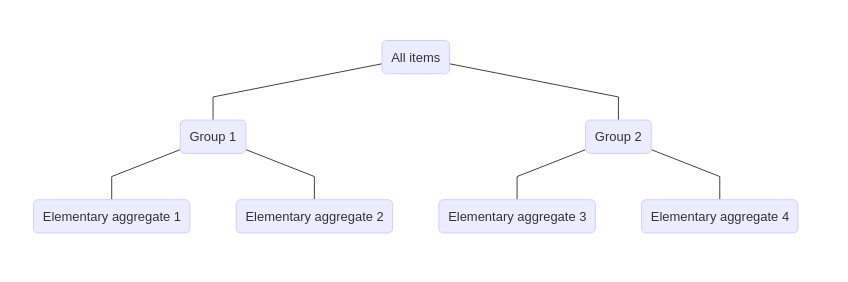
\includegraphics{img/plot1.png}

A hierarchical structure does not pose any special challenges for making a price index---one of the index-number formulas from the previous section can always be used to aggregate the price relatives for the goods and services in each group of the hierarchy to produce a collection of price indices for each level in the hierarchy. The index calculation simply needs to be repeated for each group of goods and services in the aggregation structure. This is the direct approach to calculating a price index with a hierarchical structure.

Having a hierarchical structure, however, suggests that the calculation can be simplified with a two-step procedure. In the first step, price relatives are combined at the lowest level of aggregation using one of the index-number formulas from the previous section. This gives a collection of price indices called elementary (or elemental) indices. These price indices give the movement in price over time for small, relatively homogeneous groups of goods and services called elementary aggregates that form the basis of a price index. Once the elementary indices have been calculated, indices for higher levels of aggregation are calculated by combining elementary indices using weights. These weights provide a measure of the economic importance of the goods and services in each elementary aggregate in order to combine elementary indices together to form a higher-level index. If the target index is an arithmetic index, then the elementary aggregates should be combined with a weighted arithmetic average; otherwise, if a geometric index is the target index, a weighted geometric averaged should be used. Put differently, each elementary aggregate is treated as a single good, with the elementary indices being the price relatives for these goods, and this information is fed into an index-number formula to produce a higher-level index.

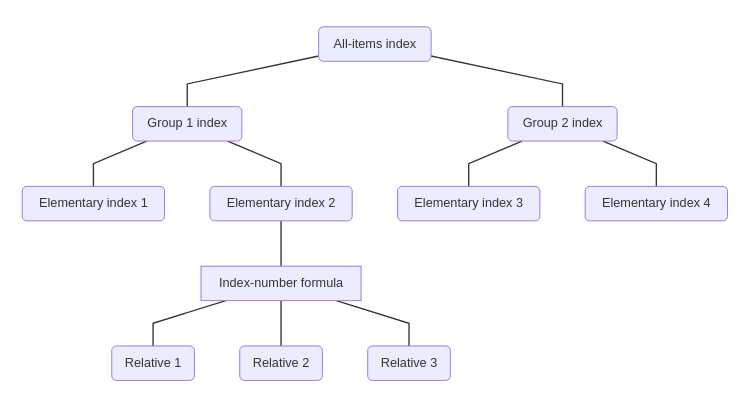
\includegraphics{img/plot2.png}

Given that there are two ways to calculate a price index with a hierarchical structure, does the direct calculation give the same result as the two-step calculation? The answer is yes for an arithmetic or geometric index, provided the weights used to aggregate the elementary aggregates are formed using the underlying weights for the target index. For example, if the goal is to calculate a Laspeyres index, then the weight for an elementary aggregate should be the expenditure/revenue share for the goods in that elementary aggregate in period 0. As both geometric and arithmetic indices are calculated as weighted averages, it should not be surprising that an index can be calculated by first grouping price relatives together, calculating group-level averages, then averaging the group-level averages to form an overall average. Consequently, these indices are said to be consistent in aggregation, although not all index-number formulas are consistent in aggregation. For example, the Fisher index is not consistent in aggregation, and using the two-step procedure to calculate it will give a different answer than the direct calculation.

It is easy to show that any arithmetic index is consistent in aggregation (the reasoning for the geometric case is almost identical). Suppose that goods are partitioned into \(k=1,\ldots,m\) distinct and mutually exclusive categories---that is, there are \(m\) elementary aggregates. If category \(k\) contains \(n_{k}\) goods, then the arithmetic index for this category is

\begin{align*}
I_{k}^{A} = \sum_{i = 1}^{n_k} \frac{\omega_{ik}}{\sum_{j = 1}^{n_k} \omega_{jk}} \frac{p_{ik1}}{p_{ik0}},
\end{align*}

where \(p_{ik1} / p_{ik0}\) is the price relative of good \(i\) in category \(k\) and \(\omega_{ik}\) is the weight for good \(i\) in category \(k\). These \(m\) indices can now be aggregated together to form an overall index by taking a weighted-average of each index, with weights given by \(\omega_{k} = \sum_{j = 1}^{n_k} \omega_{jk}\), so that

\begin{align*}
I^{A} &= \sum_{k = 1}^{m} \omega_k I_{k}^{A}  \\
&= \sum_{k = 1}^{m} \omega_k \sum_{i = 1}^{n_k} \frac{\omega_{ik}}{\sum_{j = 1}^{n_k} \omega_{jk}} \frac{p_{ik1}}{p_{ik0}} \\
&= \sum_{k = 1}^{m} \sum_{i = 1}^{n_k} \omega_{ik} \frac{p_{ik1}}{p_{ik0}}.
\end{align*}

But this is exactly the same as if the arithmetic index had been calculated by pooling all price relatives together and calculating the index directly, rather than partitioning them into groups and calculating the index in two steps.

One advantage of the two-step calculation over the direct calculation is that the index-number formula used to calculate the elementary indices can differ from the index-number formula used at higher levels aggregation. It may seem odd to want to do this, but there are a number of subtle theoretical and practical reasons why a different index-number formula should be used for the elementary indices. In most applications the elementary indices are calculated using a Jevons index, partly because detailed information on quantities bought or sold may be difficult to obtain at very low levels of aggregation. Higher levels are then calculated as an arithmetic index, usually a Young or Lowe index.

\hypertarget{factoring-an-index}{%
\subsection{Factoring an index}\label{factoring-an-index}}

When calculated over many periods, a price index gives a measure of the change in prices over time relative to a fixed base period. Calculating a price index over many periods poses no new challenges---once a base period is selected, one of the index-number formulas in the previous section can be directly applied to produce an index that evolves over time by simply forming price relatives that always calculate the change in price relative to the base period. For example, the series of geometric indices computed over periods 0, 1, and 2, with period 0 as the base period, is

\begin{align*}
1, \prod_{i = 1}^{n} \left(\frac{p_{i1}}{p_{i0}}\right)^{\omega_{i}}, \prod_{i = 1}^{n} \left(\frac{p_{i2}}{p_{i0}}\right)^{\omega_{i}}.
\end{align*}

Thus the period 1 index value gives the change in prices between period 1 and period 0, and the period 2 index gives the change in prices between period 2 and period 0. The period 0 value is 1 because the ratio of period 0 prices to period 0 prices is always 1.

Most price indices are calculated frequently---usually monthly or quarterly---and it is useful to be able to calculate a price index using only the previous period's index value and the most recent price relatives for each good covered by the index.\footnote{One reason is that it can make sampling price information easier, as the same units don't need to be sampled in both the current period and base period.} That is, it is useful to be able to factor an index into two terms: the previous period's index value, and an index that depends on only the current-period prices and previous-period prices. Such a factorization allows for an index to be calculated period-by-period, and saves from having to hold onto the price data in the base period for the life of an index. This is practically significant, as it means that an index can still be produced even if base-period price data are lost.

Factoring a geometric index is trivial; for a given set of weights, the geometric index that runs from period 0 to period \(t\) can always be written as the product of the geometric index that runs for period 0 to period \(k\) and the geometric index that runs from period \(k\) to period \(t\). That is,

\begin{align*}
I^{G}(0, t) &= \prod_{i = 1}^{n} \left(\frac{p_{it}}{p_{i0}}\right)^{\omega_i} \\
&= \prod_{i = 1}^{n} \left(\frac{p_{ik}}{p_{i0}}\right)^{\omega_i} \times \prod_{i = 1}^{n} \left(\frac{p_{it}}{p_{ik}}\right)^{\omega_i} \\
&= I^{G}(0, k) \times I^{G}(k, t).
\end{align*}

This should be deeply intuitive. If prices increased by 20\% between period 0 and period \(k\), and then increase by another 10\% between period \(k\) and period \(t\), the total increase in price from period 0 to period \(t\) is 32\%. This is the same as multiplying an index value of 1.2 by an index value of 1.1, as the result is 1.32.

Factoring an arithmetic index is slightly more complex, as it requires changing the weights used to aggregate price relatives. The arithmetic index that runs from period 0 to period \(t\) can be written as

\begin{align*}
I^{A}(0, t) &= \sum_{i = 1}^{n} \omega_{i} \frac{p_{it}}{p_{i0}} \\  
&= I^{A}(0, k) \times \sum_{i = 1}^{n} \tilde{\omega}_{i} \frac{p_{it}}{p_{ik}},
\end{align*}

where

\begin{align*}
\tilde{\omega}_{i} = \frac{\omega_{i} \frac{p_{ik}}{p_{i0}}}{I^{A}(0, k)}. 
\end{align*}

Unlike the geometric index, factoring an arithmetic index requires changing the weights for the index running from period \(k\) to \(t\). Sometimes this gets called price updating the weights, but this terminology is used inconsistently. Despite this wrinkle, however, the basic idea is the same as in the geometric case---an arithmetic index can always be decomposed into two arithmetic indices.

Intuitively, factoring an index simply tinkers with value of the index in the base period so that it can continue from a previous value without needing to be recalculated from the start. Rather than starting the index at the value 1 in period \(k\), it starts from the value of the index in period \(k\), essentially building on the cumulative change in price up to that point in time.

\hypertarget{rebasing}{%
\subsection{Rebasing}\label{rebasing}}

The base period is an important point in time for a price index, as it gives the fixed reference point to which price changes are measured against. Having to choose a base period at all, however, introduces a potential problem: what works as a base period for one use of a price index may not work for another. Fortunately, the choice of base period doesn't have much impact on the economic content of a price index---in most cases a new base period can be chosen for an index without needing to recompute the entire index series.

For a geometric index, the choice of base period has no impact on the economic content of a price index---the change in price between any two periods is the same regardless of the base period. The base period simply standardizes the index to a particular level. This can be seen by recalling that a geometric index can always be factored into two geometric indices. Given an index series with period 0 as the base period, the index value in period \(t\) with period \(k\) as the base period can always be found by simply dividing the index value in period \(t\) by the index value in period \(k\)

\begin{align*}
I^{G}(k, t) &= \prod_{i = 1}^{n} \left(\frac{p_{it}}{p_{ik}}\right)^{\omega_{i}} \\
&= \frac{\prod_{i = 1}^{n} \left(\frac{p_{it}}{p_{i0}}\right)^{\omega_{i}}}{\prod_{i = 1}^{n} \left(\frac{p_{ik}}{p_{i0}}\right)^{\omega_{i}}} \\
&= \frac{I^{G}(t, 0)}{I^{G}(k, 0)}.
\end{align*}

Hence, dividing through the index series by the period \(k\) index value produces an index series that is the same as if period \(k\) were originally chosen as the base period. This is known as rebasing an index, and means that a change in price between two periods can be computed by simply scaling the price index. This also explains why the base period gets a value in the index series, for otherwise the index series would shrink each time the index is rebased.

The chart below gives an example of how rebasing changes the time series. The index with a base period of December is simply the index with a base period of January divided by the value of the index in December (105). This simply shifts the index with January as the base period down, and squashes it a little, but does not change the relative shape of the time series.

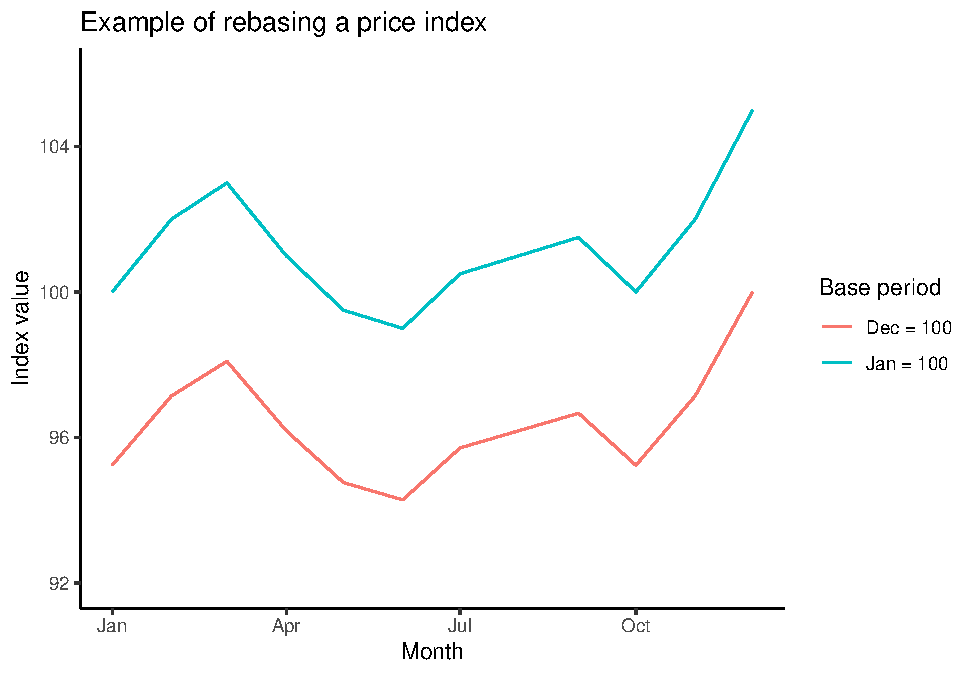
\includegraphics{price-index-course_files/figure-latex/unnamed-chunk-6-1.pdf}

Rebasing is more complex for an arithmetic index. While it works for a Lowe and Dutot index in the exact same way as a geometric index, in general rebasing an arithmetic index changes the weights used to average price relatives because of the way an arithmetic index is factored. The rebased index is still an arithmetic index, but the weights are no longer correct. For example, rebasing a Laspeyres index changes the weights so that they are no longer the base-period expenditure shares---the index is still an arithmetic index (a Lowe index), but products that have seen a larger increase in price since the base period will receive more weight in the index calculation. In practice, however, this theoretical wrinkle is usually ignored, and an arithmetic price index gets rebased by simply dividing the entire index series by the index value in the new base period.

\hypertarget{chaining}{%
\subsection{Chaining}\label{chaining}}

The weights for an index ideally give a measure of the economic importance of the goods that comprise the index, so that price relatives for goods and services with greater economic importance have a larger influence on the overall price movement between periods. In application the weights are often reused over time, as it is costly and time consuming to continuously update the weights. Keeping the same weights period after period, however, means that the weights will eventually become out of date, and may fail to capture changes in the economic importance of certain goods. Chaining an index provides a way to update the weights for an index and append new index values to the index series calculated with the old weights, without having to revise the old index series. Chaining can also be used to change the composition of goods and services covered by a price index, and this can change as new goods are introduced into a market and old goods disappear.

The idea behind chaining is the same as that for factoring an index---break an index into two pieces that can be glued together at a common overlap period. The difference is that while factoring an index is simply a trick of algebra, chaining an index is a practical solution for producing an index with a longer time series, rather than restarting the index in the period when the weights change. In both cases the idea is to modify the value in the base period of an index to reflect the cumulative change in price up to that point in time.

The steps for chaining any kind of index are the same, so consider an arithmetic index running from period 0 to period \(t\), and suppose the weights for this index change in some period \(k\). This could be because the previous weights have become sufficiently out-of-date that they need to change, or goods and services for which the index applies have changed. Whatever the reason, this gives rise to two indices, one running from period 0 to period \(k\), using period-0 weights

\begin{align*}
I^{A}(0, k) = \sum_{i = 1}^{n} \omega_{i0} \frac{p_{ik}}{p_{i0}},
\end{align*}

and another running from period \(k\) to period \(t\) using period-\(k\) weights

\begin{align*}
I^{A}(k, t) = \sum_{i = 1}^{m} \omega_{ik} \frac{p_{it}}{p_{ik}}.
\end{align*}

The chained index simply multiplies these two indices together, so that

\begin{align*}
I^{A}(0, t) = \sum_{i = 1}^{n} \omega_{i0} \frac{p_{ik}}{p_{i0}} \times \sum_{i = 1}^{m} \omega_{ik} \frac{p_{it}}{p_{ik}}.
\end{align*}

The chart below gives an example of what a chained index looks like.

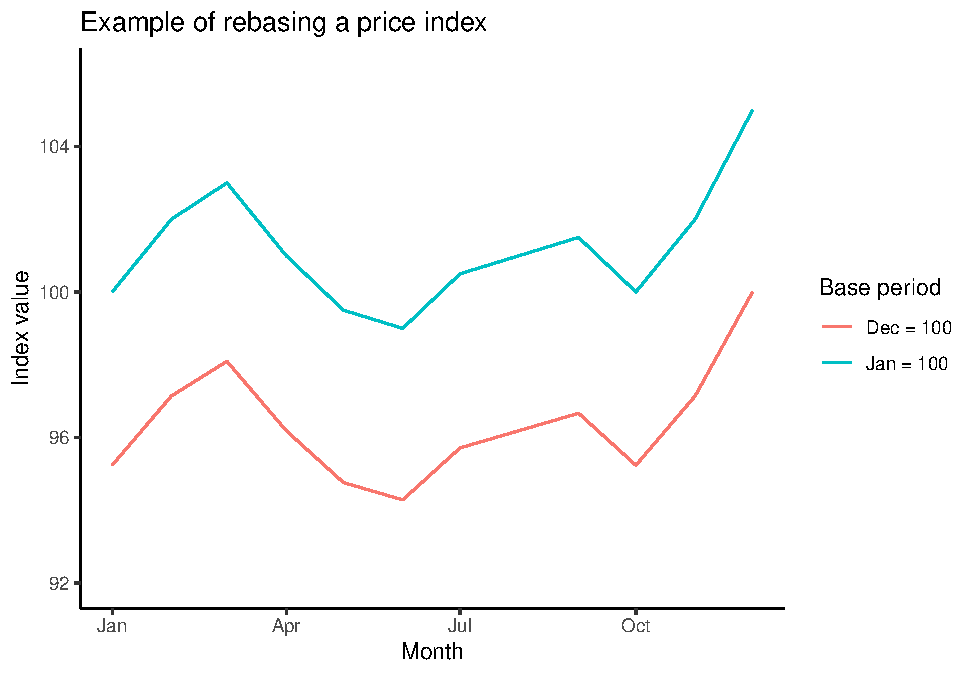
\includegraphics{price-index-course_files/figure-latex/unnamed-chunk-7-1.pdf}

The important part about a chained index is the overlap period \(k\) when the weights change, and the prices in period \(k\) get used with two sets of weights. If there is no overlap period then the index cannot be chained. Each index can be thought of as a link in the chain, giving the movement in prices for that section of time, and the overlap period is where the links meet.

\hypertarget{example-with-r-1}{%
\subsection{Example with R}\label{example-with-r-1}}

It is useful to finish this section of the course with a couple examples in R. The first example shows that a geometric index is consistent in aggregation. Calculating the index in two steps gives the same answer as the direct calculation.

\begin{Shaded}
\begin{Highlighting}[]
\CommentTok{# Bring in ppd library}
\KeywordTok{library}\NormalTok{(ppd)}

\CommentTok{# Make some price relatives}
\NormalTok{dat <-}\StringTok{ }\KeywordTok{data.frame}\NormalTok{(}\DataTypeTok{relatives =} \KeywordTok{c}\NormalTok{(}\FloatTok{1.1}\NormalTok{, }\FloatTok{1.2}\NormalTok{, }\FloatTok{0.9}\NormalTok{, }\FloatTok{1.1}\NormalTok{),}
                  \DataTypeTok{weight =} \KeywordTok{c}\NormalTok{(}\FloatTok{0.25}\NormalTok{, }\FloatTok{0.3}\NormalTok{, }\FloatTok{0.3}\NormalTok{, }\FloatTok{0.15}\NormalTok{),}
                  \DataTypeTok{group =}\NormalTok{ letters[}\KeywordTok{c}\NormalTok{(}\DecValTok{1}\NormalTok{, }\DecValTok{1}\NormalTok{, }\DecValTok{2}\NormalTok{, }\DecValTok{2}\NormalTok{)]}
\NormalTok{)}
\NormalTok{dat}
\end{Highlighting}
\end{Shaded}

\begin{verbatim}
##   relatives weight group
## 1       1.1   0.25     a
## 2       1.2   0.30     a
## 3       0.9   0.30     b
## 4       1.1   0.15     b
\end{verbatim}

\begin{Shaded}
\begin{Highlighting}[]
\CommentTok{# Calculate geometric index for group a and b relatives}
\NormalTok{index_ab <-}\StringTok{ }\KeywordTok{sapply}\NormalTok{(}\KeywordTok{split}\NormalTok{(dat, dat}\OperatorTok{$}\NormalTok{group), }
                   \ControlFlowTok{function}\NormalTok{(x) }\KeywordTok{geomean}\NormalTok{(x}\OperatorTok{$}\NormalTok{relatives, x}\OperatorTok{$}\NormalTok{weight) }\OperatorTok{*}\StringTok{ }\DecValTok{100}
\NormalTok{                   )}
\NormalTok{index_ab}
\end{Highlighting}
\end{Shaded}

\begin{verbatim}
##         a         b 
## 115.34655  96.22603
\end{verbatim}

\begin{Shaded}
\begin{Highlighting}[]
\CommentTok{# Aggregate lower-level indices}
\NormalTok{index_top <-}\StringTok{ }\KeywordTok{geomean}\NormalTok{(index_ab, }\KeywordTok{tapply}\NormalTok{(dat}\OperatorTok{$}\NormalTok{weight, dat}\OperatorTok{$}\NormalTok{group, sum))}
\NormalTok{index_top}
\end{Highlighting}
\end{Shaded}

\begin{verbatim}
## [1] 106.3125
\end{verbatim}

\begin{Shaded}
\begin{Highlighting}[]
\CommentTok{# Same as the direct calculation}
\KeywordTok{geomean}\NormalTok{(dat}\OperatorTok{$}\NormalTok{relatives, dat}\OperatorTok{$}\NormalTok{weight) }\OperatorTok{*}\StringTok{ }\DecValTok{100}
\end{Highlighting}
\end{Shaded}

\begin{verbatim}
## [1] 106.3125
\end{verbatim}

The second example shows how to rebase a price index---simply divide the index series by the value of the index in the new base period.

\begin{Shaded}
\begin{Highlighting}[]
\CommentTok{# Make an index over 12 periods with period 0 = 100}
\NormalTok{index <-}\StringTok{ }\KeywordTok{data.frame}\NormalTok{(}\DataTypeTok{period =} \DecValTok{0}\OperatorTok{:}\DecValTok{11}\NormalTok{, }\DataTypeTok{value =} \KeywordTok{c}\NormalTok{(}\DecValTok{100}\NormalTok{, }\KeywordTok{sample}\NormalTok{(}\DecValTok{90}\OperatorTok{:}\DecValTok{130}\NormalTok{, }\DecValTok{11}\NormalTok{)))}
\NormalTok{index}
\end{Highlighting}
\end{Shaded}

\begin{verbatim}
##    period value
## 1       0   100
## 2       1   121
## 3       2   105
## 4       3   129
## 5       4   128
## 6       5   104
## 7       6   102
## 8       7   101
## 9       8   106
## 10      9    97
## 11     10   107
## 12     11   123
\end{verbatim}

\begin{Shaded}
\begin{Highlighting}[]
\CommentTok{# Rebase the index so that period 6 = 100}
\KeywordTok{transform}\NormalTok{(index, }\DataTypeTok{value =}\NormalTok{ value }\OperatorTok{/}\StringTok{ }\NormalTok{value[period }\OperatorTok{==}\StringTok{ }\DecValTok{6}\NormalTok{] }\OperatorTok{*}\StringTok{ }\DecValTok{100}\NormalTok{)}
\end{Highlighting}
\end{Shaded}

\begin{verbatim}
##    period     value
## 1       0  98.03922
## 2       1 118.62745
## 3       2 102.94118
## 4       3 126.47059
## 5       4 125.49020
## 6       5 101.96078
## 7       6 100.00000
## 8       7  99.01961
## 9       8 103.92157
## 10      9  95.09804
## 11     10 104.90196
## 12     11 120.58824
\end{verbatim}

\hypertarget{assignment}{%
\section{Assignment}\label{assignment}}

Answers for these questions come from both the course content and the readings. Each question is worth one point, for a total of 20 points. Passing this module requires at least 65\% (13 out of 20 correct). Email your answers to the course instructor when you are finished.

\textbf{Question 1} True or false: The Jevons index is always smaller than or equal to the Laspeyres index.

\textbf{Question 2} Why is the Laspeyres index always larger than the Paasche index?

\begin{enumerate}
\def\labelenumi{\alph{enumi})}
\item
  Substitution bias.
\item
  Quantities are measured less precisely in the Paasche index, so the sampling variation is
  larger.
\item
  Seasonal patterns of consumption are over-estimated in the Laspeyres index.
\item
  The Laspeyres index can be smaller than the Paasche index.
\item
  None of the above.
\end{enumerate}

\textbf{Question 3} Which of the following are uses of a producer price index?

\begin{enumerate}
\def\labelenumi{\alph{enumi})}
\item
  Indicator of inflationary trends for producer inputs.
\item
  National accounts deflator.
\item
  Indicator of inflationary trends for consumer goods and services.
\item
  Cyclical adjustment margin for the balance of payments.
\item
  a and b.
\item
  a, b, and d.
\item
  All of the above.
\end{enumerate}

\textbf{Question 4} True or false: The Jevons index is always smaller than or equal to the Carli index.

\textbf{Question 5} True or false: A consumer price index gives a measure of the overall price level faced by consumers.

\textbf{Question 6} Which of the following are uses of a consumer price index?

\begin{enumerate}
\def\labelenumi{\alph{enumi})}
\item
  Indicator of inflationary trends for consumer goods and services.
\item
  National accounts deflator.
\item
  Indicator of inflationary trends for producer outputs.
\item
  Indexation of wages.
\item
  a and b.
\item
  a, b, and d.
\item
  All of the above.
\end{enumerate}

\textbf{Question 7} What are the three types of producer price indices?

\begin{enumerate}
\def\labelenumi{\alph{enumi})}
\item
  Input price, output price, transfer price.
\item
  Input price, value added, consumer price.
\item
  Output price, gate price, value added.
\item
  Input price, output price, value added.
\item
  None of the above.
\end{enumerate}

\textbf{Question 8} What is an elementary index?

\begin{enumerate}
\def\labelenumi{\alph{enumi})}
\item
  The price of raw inputs for a firm.
\item
  The price indices for the lowest level in a hierarchy.
\item
  The individual price quotes from respondents.
\item
  The value of goods and services purchased at the lowest level in a hierarchy.
\item
  None of the above.
\end{enumerate}

\textbf{Question 9} What is the usual ranking of the Fisher, Laspeyres, Lowe, and Paasche indices in terms of their magnitude (i.e., demand decreases when price increases)?

\begin{enumerate}
\def\labelenumi{\alph{enumi})}
\item
  Laspeyres ≥ Lowe ≥ Paasche ≥ Fisher.
\item
  Lowe ≥ Laspeyres ≥ Fisher ≥ Paasche.
\item
  Paasche ≥ Fisher ≥ Laspeyres ≥ Lowe.
\item
  Fisher ≥ Lowe ≥ Laspeyres ≥ Paasche.
\item
  None of the above.
\end{enumerate}

\textbf{Question 10} True or false: Weights for aggregating an index should be based on the sample of prices used to calculate the elementary aggregates.

\textbf{Question 11} True or false: A Fisher index is seen as the best type of index because it is very timely to produce.

\textbf{Question 12} Which of the following are symmetric indices?

\begin{enumerate}
\def\labelenumi{\alph{enumi})}
\item
  Fisher, Laspeyres, Paasche.
\item
  Jevons, Lowe.
\item
  Fisher, Törnqvist.
\item
  Young.
\item
  None of the above.
\end{enumerate}

\textbf{Question 13} True or false: Both the Dutot and Jevons indices are transitive.

\textbf{Question 14} Weights for a producer price index should always be based on.

\begin{enumerate}
\def\labelenumi{\alph{enumi})}
\item
  Revenue shares.
\item
  Expenditure shares.
\item
  Value added.
\item
  Current and future revenue shares.
\item
  None of the above.
\end{enumerate}

\textbf{Question 15} True or false: All price indices can be categorized as arithmetic, geometric, or harmonic.

\textbf{Question 16} Weights for a consumer price index can come from which sources.

\begin{enumerate}
\def\labelenumi{\alph{enumi})}
\item
  Scanner data.
\item
  Survey of consumer spending.
\item
  National accounts.
\item
  Census of population.
\item
  a and b.
\item
  All of the above.
\item
  None of the above.
\end{enumerate}

\textbf{Question 17} An index has a value of 90 in January and a value of 130 in May. What is the value of the index in May if January is set as the base period?

\begin{enumerate}
\def\labelenumi{\alph{enumi})}
\item
  90.0.
\item
  100.0.
\item
  140.0.
\item
  144.4.
\item
  130.0.
\end{enumerate}

\textbf{Question 18} True or false: The Fisher index is consistent in aggregation.

\textbf{Question 19} A price index has a value of 80 in March and 90 in September. What is the percent changes in price between March and September?

\begin{enumerate}
\def\labelenumi{\alph{enumi})}
\item
  10\%.
\item
  12.5\%.
\item
  -11\%.
\item
  None of the above.
\item
  It is impossible to know without knowing the base period.
\end{enumerate}

\textbf{Question 20} You are trying to make an index for blue widgets and red widgets. The price relative for red widgets is 1.2 and the price relative for blue widgets is 0.9. The expenditure share on red widgets is 0.3 in the base period and 0.25 in the current period; the expenditure share for blue widgets is 0.7 in the base period and 0.75 in the current period. What is the value of the geometric Laspeyres index?

\begin{enumerate}
\def\labelenumi{\alph{enumi})}
\item
  98.1.
\item
  96.7.
\item
  97.4.
\item
  99.0.
\item
  97.5.
\end{enumerate}

\hypertarget{part-price-index-theory}{%
\part{Price Index Theory}\label{part-price-index-theory}}

\hypertarget{syllabus-1}{%
\section{Syllabus}\label{syllabus-1}}

Why are certain index-number formulas used to compute a price index? Answering this question requires a theory of price indices that can be used to evaluate the properties of a price index, and determine if one index number is better than another.

The goal of this module is to provide the theoretical underpinnings of a price index, with a particular focus on motivating the index-number formulas that are used in practice. By the end of the module, an individual should:

\begin{enumerate}
\def\labelenumi{\arabic{enumi}.}
\item
  Be familiar with the three theoretical approaches to develop a price index.
\item
  Know how the three approaches can be used to motivate commonly-used index numbers.
\end{enumerate}

This module is useful for both users and compilers of price indices with a basic understanding of how to construct a price index, and who would like to get a deeper understanding of why particular index-number formulas are used.

This module consists of self-directed readings, along with an assignment. In total, about 10 to 15 hours should be devoted for this module.

Prerequisites: Introduction to Price Indices, at least one intermediate micro-theory course, and at least an introductory course in probability and statistics. An advanced micro-theory course is helpful.

Evaluation for this module is based on an assignment consisting of 20 multiple-choice/true-false questions that draw on material in the course content and readings. Collaboration on the assignment is welcomed, but each person must submit their own unique work. Passing this module requires at least a 65\% on the assignment.

Readings for this module come from chapters 15--18 of the PPI manual (ILO et al. 2004b) and/or the CPI manual (ILO et al. 2004a), published by the IMF (freely available on their website), as well as the review of price-index theory by Balk (1995).

Please email the course instructor if you have any questions, or need help with any of the course material or assignment.

\hypertarget{introduction}{%
\section{Introduction}\label{introduction}}

There are three broad approaches for motivating the price-index formulas that get used in practice by statistical agencies---the axiomatic approach, the economic approach, and the stochastic approach. Each approach is useful in its own right, and all three give different perspectives and understandings for the various index-number formulas that are used to construct price indices. Taken together, these different approaches constitute a theory of price indices.

Each of the three approaches can be thought of as answering a different question about how to construct a price index. The axiomatic approach attempts to answer the question ``How can information for a collection of prices and quantities be combined to satisfy certain properties?'' This is essentially a set theoretic approach for how to best construct an index number. By contrast, the economic approach attempts to answer the question ``What should a price index measure?'' The goal with the economic approach is to use the machinery of microeconomic theory to define a price index so as to measure the experience of a change in prices for consumers and producers. The stochastic approach is more pragmatic in its scope, and attempts to answer the question ``How can information on prices be used to best predict a change in price for a good or service?'' This is essentially a question about how to best inflate and deflate prices over time.

This part of the course gives a practical introduction to each of the three approaches, focusing on how they can be used to motivate the way price indices are constructed in practice. Despite having a more practical focus, however, this material is still concerned with theory that can be quite technical. Rather than focusing on the technical details (of which there are many), the part of the course gives enough of a glimpse into the technical machinery to show what is going on, while providing the economic intuition and overarching ideas from the theory.

\hypertarget{the-axiomatic-approach}{%
\section{The axiomatic approach}\label{the-axiomatic-approach}}

A price index combines information about prices and quantities at two points in time in order to produce a ratio of prices between these points in time. Unless there is only one price at each point in time, however, there is no unique way to combine prices over time---there are an infinity of possible index-number formulas that can be used to calculate a price index. This embarrassment of riches is undesirable, as it introduces considerable choice into how a price change should be measured. The axiomatic approach attempts to solve this problem by considering a general class of price indices, and finding which members of this class satisfy certain intuitive, or reasonable, properties that a price index ought to satisfy. This is equivalent to making a normative statement about how a price index should behave---what are the fundamental axioms that define a price index? The idea is to start with a very broad class of possible index-number formulas, and define axioms to whittle away index-number formulas that don't behave as a price index should.

The ideal outcome from the axiomatic approach is a single, unique index-number formula that satisfies a minimal set of uncontroversial conditions that a price index ought satisfy. This would mean that there is only one index-number formula that should be used to make a price index. The reality, however, is that compromises must be made, and keeping certain conditions requires ignoring others. Consequently, a distinction is made between axioms---fundamental statements that any reasonable price index should satisfy---and tests, which are properties that are desirable but not as fundamental as axioms. A small set of key axioms are always maintained, whereas tests can be mutually inconsistent, and choices need to be made about which tests an index should satisfy depending on its purpose. Axioms can be seen as the first sieve to remove any unreasonable index-number formulas, with tests acting as a second sieve to further refine what is left over.

This section of the course starts the journey into price index theory by giving a brief outline of the axiomatic approach to price index theory. This has been an area of considerable study, and consequently there is a lot of interesting material that is not covered in this course. The interested reader can consult either (ILO et al. 2004a, Chapter 16) or (ILO et al. 2004b, Chapter 16) for more detail, or Balk (2008).

📖 Balk (1995), skip section 4 and appendix.

📖 PPI Manual: Chapter 1, section C.

\hypertarget{an-abstract-price-index}{%
\subsection{An abstract price index}\label{an-abstract-price-index}}

In its abstract form, a price index is a function \(I\) that takes four arguments---period 0 prices \(p_{0}\), period \(t\) prices \(p_{t}\), period 0 quantities \(q_{0}\), and period \(t\) quantities \(q_{t}\), for \(n\) distinct goods and services---and returns a single value. It is a rule that turns information on prices and quantities at two points in time into one number that summarizes the change in prices. To simplify notation, prices and quantities here are vectors of prices and quantities at a point in time; for example, with \(n\) distinct goods and services, prices in period 0 are given by \(p_0 = (p_{10}, p_{20}, \ldots, p_{n0})\). This notation is useful, as a price index is a way to distill information for many prices and quantities into a single value; for example, with 25 goods and services, the price index takes 100 pieces for information (50 prices and 50 quantities) and turns it into one piece of information. For a particular collection of prices and quantities, the index value is given by \(I(p_{t}, p_{0}, q_{t}, q_{0})\).

Most price indices can be expressed in this abstract form. For example, a Laspeyres index is simply

\begin{align*}
I(p_{t}, p_{0}, q_{t}, q_{0}) = \frac{\sum_{i=1}^{n} p_{it}q_{i0}}{\sum_{i=1}^{n} p_{i0}q_{i0}}.
\end{align*}

Index-number formulas that don't make use of quantity information require no special treatment---the index value is just independent of whatever quantities were sold. For example, the Jevons index is

\begin{align*}
I(p_{t}, p_{0}, q_{t}, q_{0}) = \prod_{i=1}^{n} \left(\frac{p_{it}}{p_{i0}}\right)^{1 / n}.
\end{align*}

While most index-number formulas fit in this abstract representation, price indices that use information in a period other than period 0 or period \(t\), such as a Lowe or Young index, do not. This is an important point, as the axiomatic approach implicitly ignores these types of price indices from the start, rather than using axioms to evaluate their reasonableness as a price index.

\hypertarget{the-axioms}{%
\subsection{The axioms}\label{the-axioms}}

There are five key axioms that any price index should satisfy for all collections of prices and quantities. These axioms can be seen as generalizing the properties of the ratio of prices between period \(t\) and period 0 for a single good or service to settings with many goods and services.

\begin{enumerate}
\def\labelenumi{\arabic{enumi}.}
\item
  \textbf{Monotonicity} \(I(p'_{t}, p_{0}, q_{t}, q_{0}) > I(p_{t}, p_{0}, q_{t}, q_{0})\) if \(p'_{t} \geq p_{t}\) and \(p'_{t} \neq p_{t}\), and \(I(p_{t}, p'_{0}, q_{t}, q_{0}) < I(p_{t}, p_{0}, q_{t}, q_{0})\) if \(p'_{0} \geq p_{0}\) and \(p'_{0} \neq p_{0}\).
\item
  \textbf{Linear homogeneity} \(I(cp_{t}, p_{0}, q_{t}, q_{0}) = cI(p_{t}, p_{0}, q_{t}, q_{0})\) for any \(c > 0\).
\item
  \textbf{Identity} \(I(p_{0}, p_{0}, q_{t}, q_{0}) = 1\).
\item
  \textbf{Homogeneity of degree zero} \(I(cp_{t}, cp_{0}, q_{t}, q_{0}) = I(p_{t}, p_{0}, q_{t}, q_{0})\) for any \(c > 0\).
\item
  \textbf{Dimensional invariance} If \(A\) is a diagonal matrix of positive numbers, then \(I(Ap_{t}, Ap_{0}, A^{-1}q_{t}, A^{-1}q_{0}) = I(p_{t}, p_{0}, q_{t}, q_{0})\).
\end{enumerate}

All of these axioms are fairly straightforward to understand from their mathematical representation, perhaps with the exception of dimensional invariance, and are quite intuitive. Monotonicity simply means that a price index is increasing in period \(t\) prices and decreasing in period 0 prices---larger period \(t\) prices produce larger index values and larger period 0 prices produce smaller index values. This seems like a necessary condition for a price index to meaningfully measure inflation, as an index that does not satisfy monotonicity can decrease when prices increase.

Linear homogeneity is probably the least intuitive of the axioms, and says that multiplying all period \(t\) prices by a constant is the same as multiplying the entire index by a constant, so that a proportional increase in prices results in a proportional increase in the index. To see why this makes sense, consider two cities (A and B) that have all the same prices in period 0. If all prices in city A increase by twice as much as prices in city B between period 0 and period \(t\), with quantities purchased remaining the same in the two cities (because relative prices are the same in both cities), then it is reasonable to say that prices in city A have increased by twice as much as in city B.

The identity axiom is simple, and states that a price index does not show a change in prices if prices do not change. Like the monotonicity axiom, this seems like a necessary requirement for a price index to measure inflation; otherwise, a price index could show a change in prices when prices do not change over time.

Homogeneity of degree zero means that multiplying all prices by a constant has no impact on an index---the currency that prices are measured in does not affect the value of a price index. An index-number formula that does not satisfy homogeneity of degree zero can give a different measure of inflation depending on the currency prices are measured in, and cannot be used to compare inflation in different countries.

Dimensional invariance looks complex, but it simply says that changing the units of measurement does not change the index value. A price index should not change if all prices are multiplied by a constant and all quantities are divided by the same constant---a price index should not depend on the units of measurement.

As an example, it is straightforward to see that the Laspeyres index satisfies all five axioms.

\begin{enumerate}
\def\labelenumi{\arabic{enumi}.}
\item
  For monotonicity,

  \begin{align*}
  I(p'_{t}, p_{0}, q_{t}, q_{0}) =  \frac{\sum_{i=1}^{n} p'_{it}q_{i0}}{\sum_{i=1}^{n} p_{i0}q_{i0}} > \frac{\sum_{i=1}^{n} p_{it}q_{i0}}{\sum_{i=1}^{n} p_{i0}q_{i0}} = I(p_{t}, p_{0}, q_{t}, q_{0}) 
   \end{align*}

  whenever each \(p'_{it} \geq p_{it}\), with at least one strictly greater. The opposite holds if each \(p'_{i0} \geq p_{i0}\), with at least one strictly greater.
\item
  For linear homogeneity,

  \begin{align*}
  I(cp_{t}, p_{0}, q_{t}, q_{0}) =  \frac{\sum_{i=1}^{n} cp_{it}q_{i0}}{\sum_{i=1}^{n} p_{i0}q_{i0}} = \frac{c\sum_{i=1}^{n} p_{it}q_{i0}}{\sum_{i=1}^{n} p_{i0}q_{i0}} = cI(p_{t}, p_{0}, q_{t}, q_{0}) 
   \end{align*}

  for any \(c > 0\).
\item
  For identity,

  \begin{align*}
  I(p_{0}, p_{0}, q_{t}, q_{0}) =  \frac{\sum_{i=1}^{n} p_{i0}q_{i0}}{\sum_{i=1}^{n} p_{i0}q_{i0}} = 1.
   \end{align*}
\item
  For homogeneity of degree zero,

  \begin{align*}
  I(cp_{t}, cp_{0}, q_{t}, q_{0}) =  \frac{\sum_{i=1}^{n} cp_{it}q_{i0}}{\sum_{i=1}^{n} cp_{i0}q_{i0}} = \frac{c\sum_{i=1}^{n} p_{it}q_{i0}}{c\sum_{i=1}^{n} p_{i0}q_{i0}} = I(p_{t}, p_{0}, q_{t}, q_{0}) 
   \end{align*}

  for any \(c > 0\).
\item
  For dimensional invariance, if

  \begin{align*}
  A = 
  \begin{bmatrix}
  a_1 & \ldots & 0 \\
  \vdots & & \vdots \\
  0 & \ldots & a_n
  \end{bmatrix}
   \end{align*}

  then

  \begin{align*}
  I(Ap_{t}, Ap_{0}, A^{-1}q_{t}, A^{-1}q_{0}) = \frac{\sum_{i=1}^{n} a_{i}p_{it}a_{i}^{-1}q_{i0}}{\sum_{i=1}^{n} a_{i}p_{i0}a_{i}^{-1}q_{i0}} = \frac{\sum_{i=1}^{n} p_{it}q_{i0}}{\sum_{i=1}^{n} p_{i0}q_{i0}} = I(p_{t}, p_{0}, q_{t}, q_{0}). 
   \end{align*}
\end{enumerate}

It should be fairly safe to say that any sensible price index should satisfy these axioms. Although there are many price indices that do, the axioms work to exclude unreasonable index-number formulas that make no sense for measuring changes in prices.

\hypertarget{counter-examples}{%
\subsection{Counter examples}\label{counter-examples}}

For the most part, it is difficult to write down a half-way decent price that does not satisfy the five axioms in the previous section. Pathological examples abound, but it is more interesting to look at reasonable cases where an index-number formula does not satisfy all the axioms.\footnote{Two interesting pathological cases have to do with failure of monotonicity for the geometric Laspeyres and Paasche indices. Although the geometric Laspeyres is always increasing in period-\(t\) prices, it can also increase in period-0 prices. Necessary for this is that \(p_{i1} / p_{i0} \geq \exp(1) I(p_{0}, p_{0}, q_{t}, q_{0}) \approx 2.72 I(p_{0}, p_{0}, q_{t}, q_{0})\) for at least one good \(i\), so that at least some goods experience a change in price that is considerably larger than the change in price for the other goods. Similarly, while the geometric Paasche is always decreasing in period-0 prices, it can also decrease in period-\(t\) prices. Necessary for this to be the case is that \(p_{i1} / p_{i0} \leq I(p_{0}, p_{0}, q_{t}, q_{0}) / \exp(1) \approx I(p_{0}, p_{0}, q_{t}, q_{0}) / 2.72\) for at least one good \(i\). See Balk (2008 Section 3.12).} Two interesting examples of reasonable price indices that do not satisfy the five axioms are the Dutot index and the median-value index (i.e., the index that takes the median price relative).

The Dutot index satisfies all axioms except dimensional invariance, whereas the mean-value index satisfies all axioms except monotonicity. To see why the Dutot index does not satisfy dimensional invariance, suppose there are only two goods (i.e., \(n = 2\)) with \(p_{1t} = 1\), \(p_{2t} = 2\), and \(p_{10} = p_{20} = 1\), with

\begin{align*}
A = 
\begin{bmatrix}
1 & 0 \\
0 & 2
\end{bmatrix}.
\end{align*}

In this case

\begin{align*}
I(Ap_{t}, Ap_{0}, A^{-1}q_{t}, A^{-1}q_{0}) = \frac{1 \times 1 + 2 \times 2}{1 \times 1 + 2 \times 1} = 5 / 3
\end{align*}

and

\begin{align*}
I(p_{t}, p_{0}, q_{t}, q_{0}) = \frac{1 + 2}{1 + 1} = 3 / 2 \neq I(Ap_{t}, Ap_{0}, A^{-1}q_{t}, A^{-1}q_{0}),
\end{align*}

thus failing the dimensional invariance axiom. This simply formalizes the well known issue with the Dutot index that all goods and services must be measured in the same units for it to be useful.

To see that the median price index does not satisfy monotonicity, suppose there are 3 goods such that \(p_{1t} = 1\), \(p_{2t} = 2\), \(p_{3t} = 3\), and \(p_{10} = p_{20} = p_{30} = 1\). The median index returns the value 2 (the median price relative). Now if \(p'_{1t} = 1\), \(p'_{2t} = 2\), and \(p'_{3t} = 4\), the median index still returns 2; prices have increased, but the index value remains the same.

\hypertarget{the-tests}{%
\subsection{The tests}\label{the-tests}}

In addition to the five axioms, there are three important tests that may be desirable for a price index to satisfy. These tests are nice-to-have properties of an index, but are not as fundamental as the axioms. They act as a way to further narrow the set of price indices that satisfy the five axioms.

Stating these tests requires the concept of a quantity index, a function \(Q\) that is identical to a price index except that the role of prices and quantities is reversed. A quantity index maps quantities and prices to produce a number, although instead of giving the change in price over time, a quantity index gives the change in physical quantities over time. A quantity index should also satisfy the five axioms (switching prices with quantities).

With a quantity index in hand, the three key tests are as follows.

\begin{enumerate}
\def\labelenumi{\arabic{enumi}.}
\item
  \textbf{Circularity test} \(I(p_{t}, p_{0}, q_{t}, q_{0}) = I(p_{k}, p_{0}, q_{k}, q_{0}) I(p_{t}, p_{k}, q_{t}, q_{k})\).
\item
  \textbf{Product test} \(I(p_{t}, p_{0}, q_{t}, q_{0}) Q(q_{t}, q_{0}, p_{t}, p_{0}) = \frac{\sum_{i = 1}^{n} p_{it}q_{it}}{\sum_{i = 1}^{n} p_{i0}q_{i0}}\).
\item
  \textbf{Consistency in aggregation} For any partition of \(n\) goods into \(k = 1, \ldots, m\) distinct groups, there is a function \(\psi\) such that \(\psi(I(p_{t}, p_{0}, q_{t}, q_{0}), V_{0}, V_{t}) = \sum_{k = 1}^{m} \psi(I(p_{kt}, p_{k0}, q_{kt}, q_{k0}), V_{k0}, V_{kt})\), where \(V_{kt} = \sum_{i = 1}^{n_{k}} p_{ikt}q_{ikt}\) is the value of the \(n_{k}\) goods for group \(k\) in period \(t\), with \(V_{t} = \sum_{k = 1}^{m} V_{kt}\) being the total value in period \(t\), and if \(I(p_{kt}, p_{k0}, q_{kt}, q_{k0}) = c\) for all \(m\) groups, then \(I(p_{t}, p_{0}, q_{t}, q_{0}) = c\).
\end{enumerate}

The circularity test is straightforward, and expresses the idea that an index between two periods can be calculated by chaining the index for consecutive periods together. The circularity test legitimizes the use of chaining when calculating an index, and using period-over-period changes in price to calculate an index with a fixed base period. It also legitimizes rebasing an index.

The product test is similarly straightforward, and says that the change in aggregate value between two periods can be decomposed into a price index and a quantity index. The product tests legitimizes the use of price indices for deflating aggregate values in a national accounting framework.

The consistency in aggregation test looks complicated, but expresses a simple idea: a price index should be an aggregate of sub-indices, where aggregation depends on only the index itself and the total value of the goods for each sub-index. Consistency in aggregation legitimizes the hierarchical calculation of a price index, where price indices are calculated for increasingly broad categories of goods using the same index-number formula throughout, with value shares as weights.

As an example, the Laspeyres index satisfies the product test and the consistency in aggregation test.\footnote{The Laspeyres index does not satisfy the circularity test, as a Laspeyres index would need to be multiplied with a Lowe index to return a Laspeyres index.} For the product test, let the quantity index be

\begin{align*}
Q(q_{t}, q_{0}, p_{t}, p_{0}) = \frac{\sum_{i = 1}^{n} p_{it}q_{it}}{\sum_{i = 1}^{n} p_{it}q_{i0}},
\end{align*}

(this is the Paasche quantity index) so that

\begin{align*}
I(p_{t}, p_{0}, q_{t}, q_{0}) Q(q_{t}, q_{0}, p_{t}, p_{0}) &= \frac{\sum_{i = 1}^{n} p_{it}q_{i0}}{\sum_{i = 1}^{n} p_{i0}q_{i0}} \frac{\sum_{i = 1}^{n} p_{it}q_{it}}{\sum_{i = 1}^{n} p_{it}q_{i0}} \\
&= \frac{\sum_{i = 1}^{n} p_{it}q_{it}}{\sum_{i = 1}^{n} p_{it}q_{i0}}.
\end{align*}

For the consistency in aggregation test, let \(\psi(I(p_{t}, p_{0}, q_{t}, q_{0}), V_{0}, V_{t}) = V_0 I(p_{t}, p_{0}, q_{t}, q_{0})\), so that the test becomes

\begin{align*}
I(p_{t}, p_{0}, q_{t}, q_{0}) = \sum_{k = 1}^{m} \frac{V_{k0}}{V_0} I(p_{kt}, p_{k0}, q_{kt}, q_{k0}).
\end{align*}

The Laspeyres index obviously satisfies this condition as \(V_{k0} / V_0\) is the period-0 expenditure/revenue share for the products in group \(k\).

\hypertarget{an-impossibility-result}{%
\subsection{An impossibility result}\label{an-impossibility-result}}

Ideally there would be a single price index that satisfies the five axioms and three tests of the previous sections. This would mean that there is only one index-number formula that should ever be used, at least for the purposes of creating national statistics. However, it can be shown that there is no price index that satisfies the identity axiom, the circularity test, and the product test (Balk 1995, Theorem 1), and so \emph{a fortiori} there is no index that satisfies all five axioms and all three tests. This is because there is a trade-off between having an index that can be chained across successive periods (circularity test), and an index that fits in a national accounting framework (product test). Thus, the usefulness of a particular test depends on the use of the index, and this matters for selecting a best index in the axiomatic framework.

\hypertarget{motivating-the-jevons-and-laspeyres-indices}{%
\subsection{Motivating the Jevons and Laspeyres indices}\label{motivating-the-jevons-and-laspeyres-indices}}

Although there is no index that satisfies all five axioms and all three tests, the five axioms, along with the circularity test, uniquely define a price index as being a geometric price index with weights that do not change over time (Balk 1995, Theorem 11 and Remark 11.1). That is, a price index satisfies the five axioms and the circularity test if and only if

\begin{align*}
I(p_{t}, p_{0}, q_{t}, q_{0}) = \prod_{i = 1}^{n} \left(\frac{p_{it}}{p_{i0}}\right)^{\omega_{i}},
\end{align*}

where \(\sum_{i = 1}^{n} \omega_{i} = 1\). Note that constancy of the weights over time rules out the Törnqvist index.

Switching out the circularity test for the product test, the arithmetic Laspeyres and Paasche indices are the only indices that satisfy the five axioms, the product test, and the consistency in aggregation test (Balk 1995, Corollary 16). That is, the price index must either be

\begin{align*}
I(p_{t}, p_{0}, q_{t}, q_{0}) = \frac{\sum_{i = 1}^{n} p_{it}q_{i0}}{\sum_{i = 1}^{n} p_{i0}q_{i0}}
\end{align*}

or

\begin{align*}
I(p_{t}, p_{0}, q_{t}, q_{0}) = \frac{\sum_{i = 1}^{n} p_{it}q_{it}}{\sum_{i = 1}^{n} p_{i0}q_{it}}.
\end{align*}

These stark results help to motivate the use of these simple indices, and give some practical guidance for when to use them. A geometric index is useful when chaining an index is relatively more important than deflating aggregate values, whereas an arithmetic Laspeyres (or Paasche) index is useful when deflating aggregate values in a national accounting framework is relatively more important than using a chained calculation. This helps to explain why price indices produced by statistical agencies tend to use a geometric index for calculating elemental indices, and an arithmetic index for calculating higher-level indices. At the lowest level in an index's hierarchy, it is important to be able to calculate the elemental indices using period-over-period changes in price, but these indices don't tend to be used for deflating aggregate values. At higher levels of aggregation, there is a need to be able to deflate aggregate values, but no need for chaining period-over-period changes in price to calculate the index, as it is aggregated up from the elemental indices.

It is worth remarking that the Fisher index usually comes out as the theoretical ideal in an axiomatic framework.\footnote{Or sometimes the Törnqvist or Walsh indices, depending on the particular axioms---see Balk and Diewert (2001) and Balk (2008 Sections 3.6.4 and 3.6.5.).} This occurs because the product test is maintained without requiring consistency in aggregation, as well as imposing some other tests. Consequently, the Fisher index may be more appropriate if a price index is not calculated using a hierarchical structure. But it is important to note that this is not a foregone conclusion---one of the key results from the axiomatic approach is the ideal price index depends on its purpose, and there do not exist any universally applicable price indices.

\hypertarget{the-economic-approach}{%
\section{The economic approach}\label{the-economic-approach}}

The axiomatic approach to constructing a price index revolves around finding a way to combine information on prices and quantities in order to satisfy certain conditions. The focus is essentially set theoretic, and the goal is to define a relationship between prices over time that has the properties a price index ought to have. Except for perhaps the product test, there is no economic content to the axiomatic approach---it is a purely mathematical exercise. The economic approach, by contrast, seeks to examine the underlying economic phenomenon that a price index should measure, using the microeconomic theory of a representative, competitive firm (for a producer price index) or a representative consumer (for a consumer price index). Exactly how price information should be combined to measure a change in prices over time is completely determined by the economic concept to be measured.

Although the economic approach offers a parsimonious way to construct a price index, the validity of this approach relies on making strong assumptions about firm/consumer behavior and market conditions. The most important---and perhaps strongest---assumption is that there is a single, representative firm or consumer in the market with no market power (i.e., takes market prices as given). Having a representative firm is not a restrictive assumption if the market is competitive, but competitive behavior is indispensable (ILO et al. 2004b, Chapter 18).\footnote{The firm is also assumed to make choices to maximize profitability. Although not a controversial assumption, this need not be the only motivation for the firm---see Martin (2019).} This is problematic as most markets are characterized by some degree of imperfect competition, causing the theory to fall apart. Conversely, having a consumer take prices as given is a standard assumption, but having a representative consumer is difficult to justify, and cannot be easily relaxed (Pollak 1980; Kirman 1992).\footnote{The representative consumer is assumed to choose consumption to maximize utility. Although a standard assumption, it is becoming less accepted over time as behavioral considerations are becoming part of microeconomic theory.} Consequently, the economic approach is best seen as a consistent way to conceptualize a price index, rather than a recipe for finding an economically-superior price index, and is the least applicable of the three approaches.

This section of the course gives a brief introduction to the economic approach. As with the axiomatic approach, the focus is on motivating index-number formulas used in practice, and there is a good deal of interesting material that is not covered. Unlike the axiomatic approach, different types of indices require separate analysis because they're measuring different economic phenomena.

📖 PPI Manual: Chapter 1, section E; Chapter 17, paragraphs 17.1--17.26 and 17.61--17.67.

📖 CPI Manual: Chapter 1, paragraphs 1.85--1.107.

\hypertarget{input-price-index}{%
\subsection{Input-price index}\label{input-price-index}}

The goal of an input-price index is to measure the change in the cost of a representative firm's intermediate inputs, holding outputs fixed at some reference level. This is analogous to a fixed-basket index, except now the economic conditions facing the firm are held fixed, rather than the quantity of inputs used. This distinction is practically important, and means that there are no limits on the firm's ability to substitute more expensive inputs for less expensive inputs when prices change. An input-price index can alternatively be thought of as a cost-of-production index, analogous to a cost-of-living index for a consumer price index---an input-price index measures the firm's experience of a change in input prices.

To fix notation, let \(y\) be the amount of output a firm produces, \(q\) be the quantity of inputs available, and \(p\) the price of primary inputs. As with the axiomatic approach, these are vectors of values (i.e., \(y\) is a vector with the quantity of each output the firm produces). Taking \(y\) as fixed, and assuming the firm has no market power in the inputs market (so that the firm treats \(p\) as fixed), a profit-maximizing firm will choose its inputs, \(q\), to minimize the cost of achieving outputs \(y\). The result of this exercise is the firm's expenditure function, \(e(p, y)\), that gives the minimum cost for purchasing the inputs required to produce \(y\) units of output.\footnote{Formally, \(e(p, y) = \min_{q \in V(y)} p \cdot q\), where \(V(y)\) is the set of inputs that produce at least \(y\) units of output. This function is well-defined under fairly mild regularity conditions on the set \(V(y)\) (namely that is it non-empty and closed)---see McFadden (1978).} Because the firm is a profit-maximizer, this minimum cost of product will agree with their actual cost of production under different configurations of prices for inputs and outputs produced.

Having defined the firm's expenditure function, it is then simple to define an input cost index between period 0 and period \(t\) as

\begin{align*}
I^{C} = \frac{e(p_{t}, y_{0})}{e(p_{0}, y_{0})},
\end{align*}

where \(y_{0}\) is the amount of output produced by the firm in period 0. The input-price index measures a change in input prices by comparing the expenditure required to satisfy a fixed set of economic (output) conditions over time.

There is actually an entire family of input-price indices depending on the level at which quantities are fixed in the expenditure function. The input-price index defined above is a Laspeyres-like input-price index because the economic conditions facing the firm are fixed at their period 0 values; a Paasche-like index fixes output at its period-\(t\) level. However, the intuition is the same in all cases, so attention is restricted to the Laspeyres-like input-price index above to keep the presentation simple.

It is helpful to understand how the input-price index differs from a Laspeyres index in order to appreciate the economic approach to constructing a price index. It is easy to see that

\begin{align*}
e(p_{0}, y_{0}) = \sum_{i = 1}^{n} p_{i0} q_{i0};
\end{align*}

the value of the period-0 expenditure function is simply the observable expenditure on inputs in period 0, for otherwise the firm couldn't be operating to maximize profit in period 0. Now, in period \(t\),

\begin{align*}
e(p_{t}, y_{0}) \leq \sum_{i = 1}^{n} p_{it} q_{i0}.
\end{align*}

Obviously the inputs used in period 0 are good enough to produce the amount of output in period 0, but this choice of inputs need not minimize the cost of production at period-\(t\) prices. If the price of an input increases between period 0 and period \(t\), the firm will usually substitute away from that input and use more of a relatively cheaper input in order to minimize cost while still producing \(y_{0}\) units of output. This substitution is not reflected in the choice of inputs \(q_{0}\), and so this bundle of inputs will cost more than the cost-minimizing bundle of inputs that can produce \(y_{0}\) units of output at period \(t\) prices.

These two expression can now be used to show that

\begin{align*}
\frac{e(p_{t}, y_{0})}{e(p_{0}, y_{0})} = \frac{e(p_{t}, y_{0})}{\sum_{i = 1}^{n} p_{i0} q_{i0}} \leq \frac{\sum_{i = 1}^{n} p_{it} q_{i0}}{\sum_{i = 1}^{n} p_{i0} q_{i0}}.
\end{align*}

The Laspeyres index thus overstates the price movement between period 0 and period \(t\) because it does not take into account the substitution of inputs from a change in price that features as part of the input-price index---there is a positive substitution bias. This is the key insight from the economic approach---there is a divergence between standard index-number formulas used to measure a change in price and the economic change in price---and is the impetus to derive index-number formulas that can be used to calculate the economic input-price index.

\hypertarget{output-price-index}{%
\subsection{Output-price index}\label{output-price-index}}

An output-price index is analogous to an input-price index; the only difference is that the index compares the value of output over time, rather than the cost of inputs, holding economic conditions fixed. To this end, an output-price index compares the maximum revenue a representative firm could receive at two points in time, given a fixed set inputs for production.

Modifying the notation of the previous section, let \(p\) be the price of outputs \(y\), rather than the price of inputs \(q\). Taking inputs fixed at \(q\), a profit maximizing firm chooses its outputs \(y\) to maximize revenue, given prices \(p\). This results in the firm's revenue function, \(r(p, q)\), that gives the maximum revenue the firm could earn given market prices and a fixed quantity of inputs.\footnote{Formally, \(r(p, q) = \max_{y \in Y(q)} p \cdot y\), where \(Y(q)\) is the set of outputs that produce with at most \(q\) units of input. This function is well-defined under fairly mild regularity conditions on the set \(Y(q)\) (namely that is it compact)---see McFadden (1978).} As with an input-price index, the output-price index is defined as

\begin{align*}
I^{R} = \frac{r(p_{t}, q_{0})}{r(p_{0}, q_{0})}.
\end{align*}

An output-price index measures the value of a firm's output over time, given a fixed amount of inputs.

In contrast to an input-price index, an output-price index is always larger than a Laspeyres index. In period 0, the revenue for a firm is simply

\begin{align*}
r(p_{0}, q_{0}) = \sum_{i = 1}^{n} p_{i0} y_{i0};
\end{align*}

the value of the period-0 revenue function is simply the observable revenue period 0, for otherwise the firm couldn't be operating to maximize profit in period 0. Now, in period \(t\),

\begin{align*}
r(p_{t}, q_{0}) \geq \sum_{i = 1}^{n} p_{it} y_{i0}
\end{align*}

as the firm will produce relatively more of the outputs that have increased in price, while using the same amount of inputs. The firm substitutes away from less profitable outputs, something not reflected in the firm's choice of period-0 production. Consequently,

\begin{align*}
\frac{r(p_{t}, q_{0})}{r(p_{0}, q_{0})} = \frac{r(p_{t}, q_{0})}{\sum_{i = 1}^{n} p_{i0} y_{i0}} \geq \frac{\sum_{i = 1}^{n} p_{it} y_{i0}}{\sum_{i = 1}^{n} p_{i0} y_{i0}};
\end{align*}

a Laspeyres index understates an increase in price over time because it does not take into account the substitution of outputs over time that is part of the output-price index. This is the opposite direction of substitution bias for an input-price index, and means that the direction of substitution bias depends on what the price index is trying to measure.

\hypertarget{cost-of-living-index}{%
\subsection{Cost-of-living index}\label{cost-of-living-index}}

A cost-of-living index is entirely analogous to an input-price index, except that it measures the cost to a representative consumer associated with achieving a fixed level of utility from consumption---how does a consumer's expenditure change from a change in price to keep them as well off as they were in period 0? The theory is exactly the same as an input-price index, except that outputs \(y_0\) are replaced with a measure of utility from consumption in period 0 in the expenditure function. That is, a cost of living index is

\begin{align*}
I^{C} = \frac{e(p_{t}, u_{0})}{e(p_{0}, u_{0})},
\end{align*}

where \(u_{0}\) is the consumer's utility from consumption in period 0. Other than a change in interpretation, the mechanics of a cost-of-living index are identical to an input-price index, and will not be repeated.

\hypertarget{approximating-an-economic-index}{%
\subsection{Approximating an economic index}\label{approximating-an-economic-index}}

In practice an economic price index cannot be directly calculated. There is no hope of calculating either an input price or output-price index Without knowledge of the firm's technology of production, because the form of the firms' expenditure or revenue function is unknown. The problem is even more severe for a cost-of-living index, as it requires knowledge of consumer preferences to construct the consumer's expenditure function. The best that can be done is to approximate an economic index using data on observable prices and quantities. Both the arithmetic Laspeyres and geometric Laspeyres indices offer a good approximation to either the input price, output-price index, or cost-of-living index, at least to a first-order approximation.

The argument for approximating an economic index with an arithmetic Laspeyres or geometric Laspeyres is the same for an input-price index, an output-price index, and a cost-of-living index, and so attention is restricted to approximating an input-price index. To show that the Laspeyres index approximates the input-price index, recall that

\begin{align*}
e(p_{0}, y_{0}) = \sum_{i = 1}^{n} p_{i0} q_{i0}.
\end{align*}

Now, it can be shown that the best linear approximation to the expenditure function with period \(t\) prices is

\begin{align*}
e(p_{t}, y_{0}) \approx \sum_{i = 1}^{n} p_{it}q_{i0}
\end{align*}

whenever period-\(t\) prices are not too different from period-0 prices.\footnote{This follows from Shephard's lemma (McFadden 1978), which implies that \(e(p_{t}, y_{0}) = \sum_{i = 1}^{n} p_{it}q_{i0} + \eta(p_{t} - p_{0})||p_{t} - p_{0}||\), where \(\eta(p_{t} - p_{0}) \rightarrow 0\) when \(p_{t} \rightarrow p_{0}\).} Therefore

\begin{align*}
\frac{e(p_{t}, y_{0})}{e(p_{0}, y_{0})} \approx \frac{\sum_{i = 1}^{n} p_{it} q_{i0}}{\sum_{i = 1}^{n} p_{i0} q_{i0}},
\end{align*}

at least for small price changes.

Similarly, for the geometric Laspeyres, the best linear approximation is based on

\begin{align*}
\log(e(p_{t}, y_{0})) - \log(e(p_{0}, y_{0})) \approx \sum_{i = 1}^{n} \frac{p_{i0} q_{i0}}{\sum_{j = 1}^{n} p_{j0} q_{j0}} \log\left(\frac{p_{it}}{p_{i0}} \right).
\end{align*}

Therefore

\begin{align*}
I{^C} &= \exp(\log(e(p_{t}, y_{0})) - \log(e(p_{0}, y_{0}))) \\
&\approx \exp\left( \sum_{i = 1}^{n} \frac{p_{i0} q_{i0}}{\sum_{j = 1}^{n} p_{j0} q_{j0}} \log\left(\frac{p_{it}}{p_{i0}} \right) \right) \\
&= \prod_{i = 1}^{n} \left(\frac{p_{it}}{p_{i0}} \right)^{\omega_{i0}}
\end{align*}

where \(\omega_{i0} = p_{i0} q_{i0} / \sum_{j = 1}^{n} p_{j0} q_{j0}\) is the period-0 expenditure weight for good \(i\). As a geometric index is always smaller than its corresponding arithmetic index, and the Laspeyres index is too large relative to the input-price index (i.e., the approximation error is always positive due to substitution bias), the geometric Laspeyres index will give a better approximation to the input-price index than the Laspeyres index whenever the approximation error for the geometric index is positive.

In many cases the Fisher or Törnqvist index offers an even better approximation to an input-price index than the Laspeyres or geometric Laspeyres index. The argument for why these indices can be a better approximation are more complex---see ILO et al. (2004a Chapter 17) and ILO et al. (2004b Chapter 17) for details. The cost for this better approximation, however, is the need for more information about period \(t\) quantities, which may or may not be available at the time when the index is actually calculated.\footnote{In certain cases these approximations are exact. A Laspeyres index will be a true input-price index if the firm has a Leontief production function; a Fisher index will also be exact in this case. Similarly, a geometric Laspeyres will be a true input-price index if the firm has a Cobb-Douglas production functions; a Törnqvist index will also be exact in this case. The Lloyd-Moulton price index is an interesting case as it is exact whenever the firm has a constant elasticity of substitution production function, but it only requires period-0 quantity information.}

\hypertarget{the-stochastic-approach}{%
\section{The stochastic approach}\label{the-stochastic-approach}}

The axiomatic and economic approaches to motivating a price index take prices as fixed. As the name suggests, the stochastic approach does not; instead, prices are treated as random, at least from the point of view of whoever is compiling the price index. This is not to say that prices are chosen or determined at random, but simply that there is a distribution of prices for goods and services transacted, and observing any given price is akin to a random draw from this distribution. The obvious benefit of this approach is that it agrees with the usual practice of calculating a price index using a sample of data, allowing for an explicit treatment of the statistical properties of a price index.\footnote{Formally, in the stochastic approach, goods and services are modeled as belonging to a probability space \((\Omega, \mathcal{F}, P)\), where \(\Omega\) is the (finite) set of goods and services that are transacted, \(\mathcal{F}\) is the power set of \(\Omega\), and \(P\) is a probability measure that gives the likelihood of observing a good or service in \(\Omega\) transacted. There is then a mapping from \(\Omega\) to \(\mathbb{R}_{+}^{2}\) that gives the price of a good in period 0 and period \(t\).}

At a conceptual level, however, the stochastic approach motivates a price index by one of its main uses: deflating and inflating prices across time. The act of deflating/inflating prices is essentially one of prediction---what would the price of a good or service be in another period?---and a price index can be motivated by examining how to pick a single value that bests predicts a change in price for a population of goods sold between two periods.

This section of the course concludes the journey into price index theory by giving a somewhat more thorough introduction to the stochastic approach than is seen elsewhere. This is because the stochastic approach is probably the most practical of the three approaches. While not as lofty as the axiomatic or economic approaches, it offers the most useful model for actually producing a price index as a macroeconomic statistic.

📖 PPI Manual: Chapter 1, section D; Chapter 16, section D.

\hypertarget{the-optimal-prediction-problem}{%
\subsection{The optimal prediction problem}\label{the-optimal-prediction-problem}}

The starting point for the stochastic approach is a distribution of \(n\) price relatives between period 0 and period \(t\), with the price relative for good \(i\) given by \(p_{it} / p_{i0}\), for the population (universe) of all \(n\) goods and services to be measured by the price index. Associated with each good \(i\) is the probability \(P_{i}\) of observing this good transacted over both periods in the population of goods measured by the index, and this in turn gives a measure of frequency for observing different values for changes in price over time. Put differently, a price relative \(p_{t} / p_{0}\) is treated as a random variable in the stochastic approach, the distribution of which depends on the underlying distribution of goods and services that form the scope of the price index.\footnote{There is a tendency to think of this distribution as being Gaussian, but doing so means that some goods and services have negative prices. In most cases price relatives cannot be distributed Gaussian.}

Given a distribution of price relatives, the best predictor of a change in price between period 0 and period \(t\) is the value \(I^{A}\) that minimizes the expected prediction error. Formally, the best predictor solves the following problem\footnote{This is a prediction problem using a quadratic loss function, to ensure that the prediction error is always positive, and to formalize the idea that a large misprediction is more costly than many small mispredictions. Different loss functions usually give different optimal predictors; for example, the absolute loss function returns the median as the best predictor, which finds applications for housing price indices. If price relatives are symmetrically distributed, then all symmetric, convex loss functions give the same price index (Lehmann and Casella 1998, Chapter 1 Corollary 7.19).}

\begin{align*}
\min_{I} E\left[\left(\frac{p_{t}}{p_{0}} - I \right)^{2}\right],
\end{align*}

where \(E\) is the expected value operator, taken over the distribution of price relative. As is well known, the solution to this problem is to set \(I^{A} = E(p_{t} / p_{0})\) (Lehmann and Casella 1998, Chapter 1 Example 7.17); that is, the best predictor of a change in price between two periods is the expected change in price. While it may seem unusual to express a price index in terms of an expected value, this simply emphasizes that a price index is rightfully a feature of the distribution of prices in the population. This is a key feature of the stochastic approach, and is what allows for a meaningful analysis of the statistical properties of a price index when calculated with a sample of price data from the population.

The figure gives an example of what the prediction problem looks like. Given a distribution of price relatives (solid line), there is an associated expected prediction error with each value that a price index can take (dashed line). The best choice for a price index as a predictive tool is the value that minimizes the expected prediction error (dotted line).

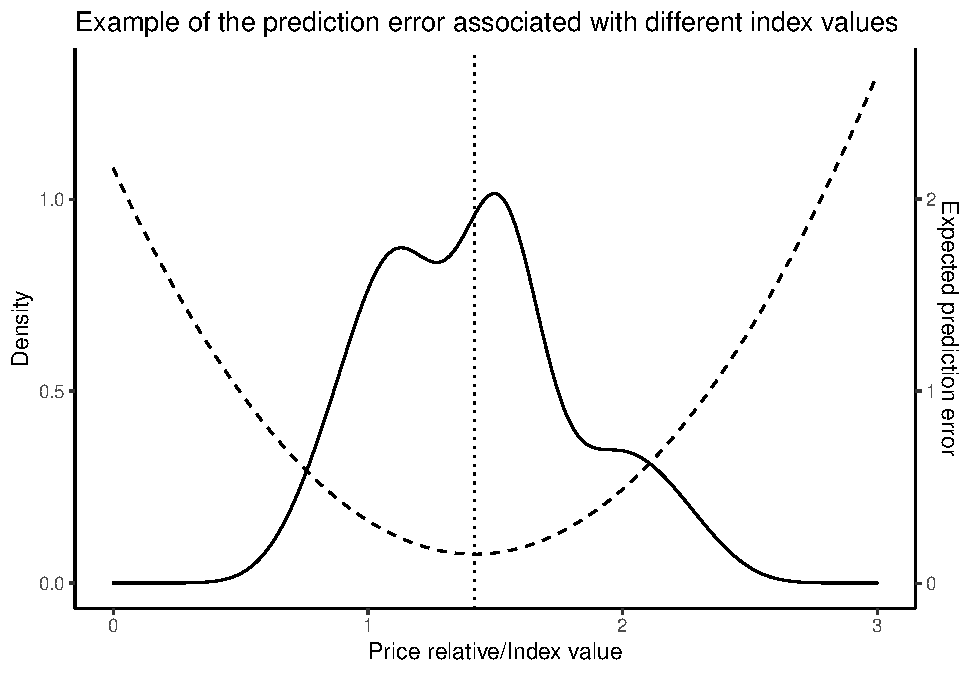
\includegraphics{price-index-course_files/figure-latex/unnamed-chunk-10-1.pdf}

As the expected value is just a weighted average, the index \(I^{A} = E(p_{t} / p_{0})\) is simply an arithmetic index that averages price relatives. What's interesting is that the weights now have a new interpretation---they are the probability of observing a good or service transacted in the population. That is,

\begin{align*}
I^{A} = \sum_{i = 1}^{n} \frac{p_{it}}{p_{i0}} P_{i}.
\end{align*}

Different arithmetic price-index formulas---e.g., Laspeyres, Paasche, Lowe---thus correspond to different statements about what determines the probability of observing a transaction. For example, with a Laspeyres index the probabilities are given by period-0 expenditure or revenue shares. This amounts to a statement that the probability of observing a transaction for a good is the likelihood of spending or receiving a dollar on that good in period 0.

\hypertarget{geometric-price-indices-1}{%
\subsection{Geometric price indices}\label{geometric-price-indices-1}}

A geometric index can be motivated in the same way as an arithmetic index. Formally, a geometric index is the value \(I^{G}\) that solves

\begin{align*}
\min_{I} E\left[\left(\log\left(\frac{p_{t}}{p_{0}}\right) - \log(I) \right)^{2}\right],
\end{align*}

the solution to which is \(I^{G} = \exp(E[\log(p_{t} / p_{0})])\). But this is just a geometric index, as

\begin{align*}
\exp\left(E\left[\log\left(\frac{p_{t}}{p_{0}}\right)\right]\right) &= \exp\left(P_{i} \sum_{i = 1}^{n} \log\left(\frac{p_{it}}{p_{i0}}\right)\right) \\
&= \prod_{i = 1}^{n} \left(\frac{p_{it}}{p_{i0}}\right)^{P_{i}},
\end{align*}

with weights equal to the probability of observing a price relative. It is worth noting that, due to the logarithms in the prediction problem, a geometric index can equally be motivated as finding a value \(I^{G}\) such that \(I^{G} \times p_{i0}\) best predicts \(p_{it}\) (or \(p_{it} / I^{G}\) best predicts \(p_{i0}\)). This is a property not shared with arithmetic indices. Whereas an arithmetic index predicts price changes over time, a geometric index takes the price for a good in period 0, inflates/deflates it with the price index, and uses the result to predict the price for that good in period \(t\). Consequently, a geometric index fits more neatly into the stochastic approach as it directly corresponds with how a price index is used to inflate and deflate prices over time in practice.\footnote{Motivating a price index as solving the problem \(\min_{I} E[(p_{t} - p_{0} I)^{2}]\) results in \(I = E(p_{t} p_{0}) / E(p_{0}^{2})\), which is a rather unusual price index.}

The Törnqvist index usually comes out as the best index in the stochastic approach because it picks a sensible value to represent the probability of observing a price relative. The idea behind the Törnqvist probabilities is that the likelihood of observing a particular price relative for a good depends on the expenditure/revenue share of that good across both periods. Thus, the Törnqvist index sets the probabilities as average expenditure shares:

\begin{align*}
P_{i} = \frac{1}{2} \frac{p_{i0}q_{i0}}{\sum_{j = 1}^{n} p_{j0}q_{j0}} + \frac{1}{2} \frac{p_{it}q_{it}}{\sum_{j = 1}^{n} p_{jt}q_{jt}}.
\end{align*}

The disadvantage of these probabilities is that they require information for both period-0 and period-\(t\) expenditure/revenue shares, something that may not be known at the time the index is calculated.

\hypertarget{more-general-price-indices}{%
\subsection{More general price indices}\label{more-general-price-indices}}

The arithmetic and geometric indices are special cases of a broader class of price indices that solve the following prediction problem:

\begin{align*}
\min_{I} E\left[\left(\left(\frac{p_{t}}{p_{0}}\right)^{r} - I^{r} \right)^{2}\right],
\end{align*}

for some \(r \neq 0\). The solution to this problem is \(I = E((p_{t} / p_{0})^{r})^{1 / r}\). Setting \(r = 1\) gives an arithmetic index, whereas taking \(r \rightarrow 0\) gives a geometric index (Bullen 2003, III 1 Theorem 2).

What's useful about this approach is that many other types of price indices correspond to different choices of \(r\), and these in turn can be motivated as solving a type of prediction problem. Setting \(r = -1\), for example, yields a harmonic price index

\begin{align*}
I^{H} = \left(\sum_{i = 1}^{n} \frac{P_{i}}{p_{it} / p_{i0}} \right)^{-1}.
\end{align*}

When the probability of observing a good is given by its period-\(t\) expenditure share, then this is the Paasche index. Setting \(r = 1 - \sigma\), where \(\sigma\) is the elasticity of substitution, results in the Lloyd-Moulton price index

\begin{align*}
I^{LM} = \left(\sum_{i = 1}^{n} P_{i} \left(\frac{p_{it}}{p_{i0}}\right)^{1 - \sigma}\right)^{1 / (1 - \sigma)}
\end{align*}

when the probabilities are period-0 expenditure/revenue shares.

An interesting point about these more general types of price indices is that, for a given set of weights, the index value is larger when the parameter \(r\) increases (Bullen 2003, III 3.1 Theorem 1). This gives the familiar result that an arithmetic index is larger than a geometric index, which in turn is larger than a harmonic index, but it can also be used to rank more exotic types of indices like the Lloyd-Moulton index.

\hypertarget{statistical-inference}{%
\subsection{Statistical inference}\label{statistical-inference}}

In practice the entire distribution of price relatives is usually not known, and an index is calculated using a sample of prices collected from producers or retailers. This means that the index values are calculated with an estimator for either \(I^{A}\) or \(I^{G}\), depending on whether an arithmetic or geometric index is the target index. Although the topics of sampling and statistical inference get complicated fast, and are beyond the scope of this course, it is worth examining how the arithmetic and geometric indices behave when calculated with a random sample of price data.\footnote{See Balk (2008 Chapter 5) for an introduction to sampling and statistical inference for price indices.} One of the benefits of the stochastic approach is that it gives insight into the problem of estimating a price index with a sample.

With random sampling, a natural approach for estimating the arithmetic index is to replace the expected value---a population average---with the sample average. This gives a method-of-moments estimator \(\hat{I}^A = 1 / n_{s} \sum_{i = 1}^{n_{s}} p_{it} / p_{i0}\), where \(n_{s}\) is the sample size, which is just a Carli index. If price relatives are sampled at random, then is it easy to see that \(E(\hat{I}^{A}) = I^{A}\), so the Carli index is an unbiased estimator for the arithmetic index.

A natural estimator for the geometric index is \(\hat{I}^{G} = \prod_{i = 1}^{n_{s}} (p_{it} / p_{i0})^{1 / n_{s}}\), the Jevons index. Unlike the Carli index, however, the Jevons index is a biased estimator of the geometric index. It is again straightforward to show that \(E(\hat{I}^{G}) \geq I^{G}\), with \(E(\hat{I}^{G}) = I^{G}\) only holding in very special circumstances---the Jevons index systematically overestimates the geometric index (i.e., it is biased upwards).\footnote{The Jevons index is not biased in cases where the sampling distribution is degenerate, or the variance in price relatives is zero. See Lehmann and Casella (1998 Chapter 1 Theorem 7.5).} Although biasedness is a disadvantage of the Jevons index, the bias is not the only important statistical property of an estimator, and the Jevons index has other desirable statistical properties (e.g., it is a consistent estimator of the geometric index, and in certain circumstances achieves the maximum likelihood efficiency bound).\footnote{The Carli index is also a consistent estimator of the arithmetic index under random sampling, but it cannot be a maximum likelihood estimator as this would require price relatives to have a Gaussian distribution, which means that price relatives can be negative. By contrast, the Jevons index is a maximum likelihood estimator for the geometric index if price relatives have a log-normal distribution, which implies that prices are always positive.} It is possible to adjust for the upwards bias in the Jevons by dividing the Jevons index by \(1 + \sigma^{2}/(2n)\), where \(\sigma^{2}\) is the variance of the log price relatives (Kennedy 2003, 41), but this is not usually done in practice.

\hypertarget{assignment-1}{%
\section{Assignment}\label{assignment-1}}

Answers for these questions come from both the course content and the readings. Each question is worth one point, for a total of 20 points. Passing this module requires at least 65\% (13 out of 20 correct). Email your answers to the course instructor when you are finished.

\textbf{Question 1} True or false: The Laspeyres index is a cost-of-living index if consumers do not substitute away from more expensive goods when prices change.

\textbf{Question 2} True or false: The time-reversal test says that a price index between period 0 and period 1 is the same as the reciprocal of the price index between period 1 and period 0.

\textbf{Question 3} What is the difference between the economic and axiomatic approaches to index numbers?

\begin{enumerate}
\def\labelenumi{\alph{enumi})}
\item
  Prices and quantities are independent in the axiomatic approach and dependent in the economic approach.
\item
  The economic approach treats prices as fixed, whereas the axiomatic approach treats prices as random.
\item
  The economic approach consists of a series of test based on economic theory to gauge the appropriateness of an index number, while the axiomatic approach uses the fundamental axioms from set theory to gauge how well an index number compares lists of prices.
\item
  The axiomatic approach and the economic approach are equivalent.
\item
  None of the above.
\end{enumerate}

\textbf{Question 4} What weights does the Palgrave index use to aggregate price relatives between period 0 and period 1?

\begin{enumerate}
\def\labelenumi{\alph{enumi})}
\item
  Period-0 expenditure/revenue shares.
\item
  Period-1 expenditure/revenue shares.
\item
  The geometric average of period-0 and period-1 expenditure/revenue shares.
\item
  The harmonic average of period-0 and period-1 expenditure/revenue shares.
\item
  None of the above.
\end{enumerate}

\textbf{Question 5} True or false: The Fisher index is highly regarded as an index number because it satisfies the most important axioms and always corresponds to a cost-of-living index.

\textbf{Question 6} True or false: The time-reversal test says that a price index and a quantity index have the same functional form.

\textbf{Question 7} Which axiom does the Dutot index not satisfy?

\begin{enumerate}
\def\labelenumi{\alph{enumi})}
\item
  Monotonicity.
\item
  Continuity.
\item
  Dimensional invariance.
\item
  Circularity.
\item
  None of the above.
\end{enumerate}

\textbf{Question 8} True or false: It is impossible for a geometric Laspeyres index to be a cost-of-living index.

\textbf{Question 9} What type of index should be used to calculate a Laspeyres quantity index by deflating the change in aggregate value between two periods?

\begin{enumerate}
\def\labelenumi{\alph{enumi})}
\item
  Palgrave index.
\item
  Laspeyres index.
\item
  Paasche index.
\item
  Fisher index.
\item
  Geometric Laspeyres index.
\end{enumerate}

\textbf{Question 10} True or false: The Jevons index is a biased estimator of the geometric index in the population under random sampling.

The next 4 questions use data in the following table that contains a population of three price relatives, each with equal probability, and all possible samples from this population.

\begin{longtable}[]{@{}llll@{}}
\toprule
Population of price relatives & Sample 1 & Sample 2 & Sample 3\tabularnewline
\midrule
\endhead
1.2 & 1.2 & 1.2 & 1.1\tabularnewline
1.1 & 1.1 & 1.35 & 1.35\tabularnewline
1.35 & \ldots{} & \ldots{} & \ldots{}\tabularnewline
\bottomrule
\end{longtable}

\textbf{Question 11} What is the value of the geometric index in the population?

\begin{enumerate}
\def\labelenumi{\alph{enumi})}
\item
  121.2
\item
  100
\item
  120.5
\item
  129.8
\item
  98.7
\end{enumerate}

\textbf{Question 12} What is the (arithmetic) average value of the Jevons indices in each sample?

\begin{enumerate}
\def\labelenumi{\alph{enumi})}
\item
  121.2
\item
  119.4
\item
  121.3
\item
  100
\item
  123.1
\end{enumerate}

\textbf{Question 13} What is the value of the bias in the Jevons index?

\begin{enumerate}
\def\labelenumi{\alph{enumi})}
\item
  0
\item
  -0.2
\item
  0.1
\item
  0.8
\item
  -1.3
\end{enumerate}

\textbf{Question 14} What is the value of the bias in the Carli index?

\begin{enumerate}
\def\labelenumi{\alph{enumi})}
\item
  1.1
\item
  -0.4
\item
  -0.2
\item
  0.7
\item
  0
\end{enumerate}

\textbf{Question 15} True or false: If a representative consumer has a constant elasticity of substitution utility function, the magnitude of the substitution bias increases as the elasticity of substitution increases.

The next four questions use data in the following table that contains information on prices and quantities for two inputs over two periods, along with a true input-price index.

\begin{longtable}[]{@{}llllll@{}}
\toprule
Period & Price 1 & Price 2 & Quantity 1 & Quantity 2 & Input-price index\tabularnewline
\midrule
\endhead
0 & 100 & 60 & 141 & 391 & 100.0\tabularnewline
1 & 120 & 80 & 160 & 360 & 128.0\tabularnewline
\bottomrule
\end{longtable}

\textbf{Question 16} What is the value of the Laspeyres index?

\begin{enumerate}
\def\labelenumi{\alph{enumi})}
\item
  101.0
\item
  133.3
\item
  128.0
\item
  128.3
\item
  99.3
\end{enumerate}

\textbf{Question 17} What is the value of the Paasche index?

\begin{enumerate}
\def\labelenumi{\alph{enumi})}
\item
  127.7
\item
  131.2
\item
  101.0
\item
  99.1
\item
  130.0
\end{enumerate}

\textbf{Question 18} What is the value of the Jevons index?

\begin{enumerate}
\def\labelenumi{\alph{enumi})}
\item
  120.1
\item
  128.2
\item
  99.0
\item
  126.5
\item
  98.4
\end{enumerate}

\textbf{Question 19} True or false: The Jevons index calculated in question 18 is closer in value to the input-price index than the Fisher index.

\textbf{Question 20} True or false: It is possible to construct an input-price index for a firm that has market power for the goods it sells.

\hypertarget{part-constant-quality-price-indices}{%
\part{Constant-Quality Price Indices}\label{part-constant-quality-price-indices}}

\hypertarget{syllabus-2}{%
\section{Syllabus}\label{syllabus-2}}

A price index should measure a pure price movement over time. In practice, however, goods and services change over time, and this can contaminate a price index---without additional information, there is no way to disentangle a price movement from a change in the quality of a good or service.

The goal of this module is to touch on some advanced topics in the construction of price indices, with a particular focus on quality adjustments and missing data. By the end of the module, an individual should:

\begin{enumerate}
\def\labelenumi{\arabic{enumi}.}
\item
  Be familiar with the need to make quality adjustments in a price index, and the link with missing data.
\item
  Understand the importance of stratification for constructing a price index.
\item
  Have a basic understanding of price indices that use econometric methods to deal with quality changes.
\end{enumerate}

This module is useful for compilers of price indices with an understanding of the basic theory and construction of a price index, and who would like to get a deeper understanding of how to deal with quality adjustments and missing data.

This module consists of self-directed readings, along with an assignment. In total, about 10 to 15 hours should be devoted for this module

Prerequisites: Price Index Theory, at least one introductory course in econometrics. An advanced course in econometrics or probability and statistics is helpful.

Evaluation for this module is based on an assignment consisting of 20 multiple-choice/true-false questions that draw on material in the course content and readings. Collaboration on the assignment is welcomed, but each person must submit their own unique work. Passing this module requires at least a 65\% on the assignment.

Readings for this module come from chapters 17 and 21 of the PPI manual (ILO et al. 2004b) and/or the CPI manual (ILO et al. 2004a), published by the IMF (freely available on their website), as well as chapter 4--6 in the Handbook on Residential Property Price Indices (ILO et al. 2013), published by Eurostat (freely available on their website).\footnote{Although the focus of the handbook is on residential property prices, the ideas are applicable to any goods or services, and the material is presented relatively well.}

Please email the course instructor if you have any questions, or need help with any of the course material or assignment.

\hypertarget{introduction-1}{%
\section{Introduction}\label{introduction-1}}

Accounting for quality differences between goods is a perennial concern when constructing a price index. The goal of a price index is to capture a pure price movement across two periods, but if there are systematic differences in the goods being compared over time that also affect price---so-called differences in quality---then a pure price movement cannot be captured using transaction prices alone. Without prior information, there is no way to disentangle a pure price movement from a movement in price due to changing quality over time. The ideal measure of a pure price movement is a constant-quality price index that holds the determinants of price fixed across periods. This allows for an apples-to-apples comparison using transaction prices, and any difference in prices between periods must reflect a pure price movement.

There are a number of techniques available to combat quality differences creeping into a price index. Probably the simplest and most intuitive approach is the pure matched-model index, wherein prices for pairs of similar goods are compared over time. By focusing on pairs of similar goods, it becomes less likely that differences in quality between different goods can contaminate measurement of a pure price movement. Other more exotic techniques, namely stratification and hedonics, offer the same promise of a constant-quality price index, usually at the expense of additional econometric apparatus.

One interesting feature of these different methods---matched model, stratification, and hedonics---is that they really aren't that different. Each relies on the same key assumption to produce a constant-quality index; what differs between the methods is simply how they go about implementing this assumption. This point is fundamental in order to understand how these different approaches can deliver a constant-quality index, and how they relate to each other.

In the interest of simplicity, this course focuses on geometric price indices. The concepts for a geometric index are directly applicable to arithmetic indices, although there are some extra details to worry about in the arithmetic case.\footnote{See Lee (2016 Chapter 1) and Manski (2007 Chapter 7) for some of the details.} In most applications quality adjustments are done using a geometric index-number formula. Throughout this course, attention is focused on building a constant-quality index when the entire population of transactions for goods and services is known. This is almost never the case in practice, but it makes the exposition easier by ignoring issues associated with sampling and statistical inference. It also emphasizes that building a constant-quality index is fundamentally a population-level problem, and not an issue of sampling. Once a constant-quality index is defined in the population, it is simple to estimate it with a sample of transactions by replacing the population-level quantities with their sample analogs---see Manski (1988).

\hypertarget{potential-prices}{%
\section{Potential prices}\label{potential-prices}}

Formalizing a constant-quality index requires extending the stochastic approach to index numbers by generalizing the concept of a price. To this end, define a potential price as the price that a good or service would sell for at a point in time, irrespective of whether it actually sells---a potential price is a counter-factual price for a good or service at a point in time. This is in contrast to a transaction price, which is the observed price that a good sells for at the point in time when it actually sells. Comparing potential prices at two points in time gives a constant-quality index, as the goods being compared are necessarily held fixed over time. This is simply a pure price movement across two periods, abstracting from changes in price due to differences in the characteristics of goods selling in these periods.

The concept of a potential price is extremely useful. In the standard price-index model, only prices and quantities can change over time. With potential prices, however, the composition of what sells over time can also change. This generalization makes it possible to define a price index when not only price and quantities change over time, but also what sells changes over time.

A potential price is a particular type of potential outcome that forms the basis of the Rubin Causal Model, a workhorse model for making causal inference in the program evaluation literature. The Rubin Causal Model revolves around the narrative of an experiment, where one group of individuals is given a treatment, with the other group serving as a controlled benchmark. The goal of the experiment is to get a measure of the causal impact of treatment. In the context of a price index, a constant-quality index is the causal effect of time on prices, and it is useful to keep the narrative of an experiment in mind. Manski (2007 Chapter 7), Angrist and Pischke (2009 Chapters 2--4), and Wooldridge (2010 Chapter 21) each provide an excellent presentation of the potential outcomes framework. Lee (2016) gives a book-length treatment.

To operationalize the concept of a potential price in the stochastic framework, suppose there are \(n\) unique goods that can sell in either period \(t = 0\) or period \(t = 1\). Let \(p_{i}(1)\) be the price of good \(i\) if it were to sell in period 1, and let \(p_{i}(0)\) be the price of good \(i\) if it were to sell in period 0, irrespective of when the good actually sells. If good \(i\) actually sells in period 1, then the price \(p_{i}(1)\) is the observed transaction price---it can be observed when the good sells in period 1---whereas \(p_{i}(0)\) is counter-factual, and hence unobservable. Similarly, if good \(i\) sells in period 0, then \(p_{i}(0)\) is the transaction price, with \(p_{i}(1)\) counter-factual. Thus for every transaction price there is also a counter-factual price, and this allows a price relative \(p_{i}(1) / p_{i}(0)\) to be constructed despite a good not selling in both periods.

Treating each good as unique and selling only once may seem odd, but it is the appropriate way to model goods over time. This means that the same product sold at two different points in time is really two different goods, and this allows the quality of the same product to change over time. For example, cat food may sell in both period 0 and period 1, but these are treated as distinct goods as the quality of cat food may change between period 0 and period 1, if, for example, the size of the can is smaller in period 1. Having each good be unique also allows products to disappear over time, or not sell in every period, and all of these issues can be treated in one framework using the concept of a potential price. Clearly this has more applicability to certain types of products (e.g., housing, computers, cars) than others (e.g., food), but the framework is sufficiently general to cover all types of goods and services.

\hypertarget{constant-quality-price-indices}{%
\subsection{Constant-quality price indices}\label{constant-quality-price-indices}}

Motivating a constant-quality price index proceeds exactly as it did in the stochastic framework, except now potential prices are used in place of transaction prices. The idea is that there is a distribution of potential price relatives, one for each good, and a price index acts as a best predictor of the change in prices over time. By using potential prices, however, the exact same goods are being compared over time, even if a product as it appears in the market changes between period 0 and period 1. Formally, a constant-quality (geometric) price index is given by

\begin{align*}
I^{Q} &= \exp\left(E\left[\log\left(\frac{p(1)}{p(0)}\right)\right]\right) \\
&= \prod_{i = 1}^{n} \left(\frac{p_{i}(1)}{p_{i}(0)}\right)^{P_{i}},
\end{align*}

where \(P_{i}\) is the probability of observing good \(i\) in the population of goods. A constant-quality index is a generalization of the standard geometric index that explicitly allows goods, as well as prices, to change over time.

In order to simplify the notation, let \(\rho(t) = \log(p(t))\). With this new notation, a constant-quality price index is given by

\begin{align*}
\log(I^{Q}) = E(\rho(1)) - E(\rho(0)).
\end{align*}

This notation is convenient because it allows a constant-quality price index to be written as a difference in average potential prices, although the index is still a geometric average of potential price relatives.\footnote{This is a Törnqvist-like index, as it gives the change in price for all goods and services transacted between period 0 and period 1. A Laspeyres-like index uses only the distribution of goods that transact in period 0, so that \(\log(I^{Q}) = E(\rho(1) | t = 0) - E(\rho(0) | t = 0)\); a Paasche-like index uses the distribution of goods that transact in period 1, so that \(\log(I^{Q}) = E(\rho(1) | t = 1) - E(\rho(0) | t = 1)\). In the language of an experiment, a Törnqvist-like constant-quality index is the average treatment effect, whereas a Laspeyres-like index is the average treatment effect on the untreated, and a Paasche-like index is the average treatment effect on the treated.}

\hypertarget{transaction-price-indices}{%
\subsection{Transaction-price indices}\label{transaction-price-indices}}

The challenge with constructing a constant-quality price index is that potential prices are not observable, and only information on transaction prices and the time when a good sells can be used to calculate an index. There is a problem of missing data. This can be seen by linking transaction prices to potential prices as

\begin{align*}
\rho = \rho(0) + t(\rho(1) - \rho(0)),
\end{align*}

where \(\rho\) is the (log) transaction price, and \(t\) gives the period of sale (either \(t = 1\) or \(t = 0\)). The only information that can be observed from market transactions is \(\rho\) and \(t\)---the price that a good sold for and the time when it actually sold.

Given information on transaction prices, a geometric transaction-price index attempts to mimic the constant-quality index by comparing the average transaction price for the goods that sell in period 1 with the average transaction price for the goods that sell in period 0, and is thus given by

\begin{align*}
\log(I^{T}) &= E(\rho | t = 1) - E(\rho | t = 0) \\
&= E(\rho(1) | t = 1) - E(\rho(0) | t = 0).
\end{align*}

The transaction-price index generally differs from the constant-quality index, as it compares potential prices for those goods that sell in period 1 to potential prices for those goods that sell in period 0, rather than for all goods. Any change in the composition of goods selling between period 0 and period 1 will contaminate the measurement of a pure price movement, as the same goods are not being compared over time. What the goods selling in period 0 sold for may differ from what the goods selling in period 1 would have sold for in period 0, so comparing average transaction price mixes up a change in price with a change in the composition of goods selling at different points in time.\footnote{Returning to the narrative of an experiment, goods that sell in period 1 are the treatment group and goods that sell in period 0 are the control group, with the transaction-price index giving the average difference in the outcome of the experiment. This may or may not correspond the causal effect of treatment, depending on how the treatment and control groups are formed. For example, suppose the treatment is visiting a hospital and the outcome is a measure of health. Simply comparing health outcomes for those that have recently visited a hospital to those that have not, while ignoring how these groups are formed, would lead one to falsely conclude that visiting a hospital makes people unhealthy as on average those who have recently visited the hospital are in worse health than those who have not. This is because those visiting a hospital were likely to have worse health outcomes anyways, hence an apples-to-orange comparison.}

Note that this index is not necessarily based on price relatives, as the same number of goods may not sell in each period. If \(n(t)\) denotes the set of goods that sell in period \(t\), the geometric transaction-price index is a ratio of geometric averages,

\begin{align*}
\log(I^{T}) = \frac{\prod_{i \in n(1)} p_{i}(1)^{P_{i}|t = 1}}{\prod_{i \in n(0)} p_{i}(1)^{P_{i}|t = 0}},
\end{align*}

where \(P_{i} | t\) is the conditional probability of observing good \(i\) in period \(t\). This is just a generalization of the usual geometric price index when different goods sell over time.

\hypertarget{identification}{%
\subsection{Identification}\label{identification}}

It is not possible to construct a constant-quality price index with only knowledge of transaction prices and when goods sell. All that can be known is the transaction-price index, which need not agree with the constant-quality index. Making progress towards identifying a constant-quality price index with information on transaction prices requires making assumptions.

If this independence assumption holds, then \(E(\rho(t) | t) = E(\rho(t))\) for \(t=0,1\) and so, as long as \(0 < P(t = 1) < 1\), so that there are goods that sell in both periods,

\begin{align*}
\log(I^{Q}) &= E(\rho(1)) - E(\rho(0)) \\ 
&= E(\rho(1) | t = 1) - E(\rho(0) | t = 0) \\
&= \log(I^{T}).
\end{align*}

That is, the constant-quality index is identical to the observable transaction-price index.\footnote{One of the key insights from the program evaluation literature is that it is often easier to get a treatment effect for a sub-population than for the entire population. For example, the average effect of treatment on the treated is identified under weaker conditions than the average treatment effect on the entire population. As a constant-quality price index is just an average treatment effect, it is worth wondering if independence can be relaxed while still delivering a constant-quality index. In certain cases the answer is yes, if a price index applies to a sub-population of goods (e.g., the population of goods that actually sell in period 1, which is the average treatment effect on the treated). This means that tools in the program evaluation literature---such as instrumental variables for local average treatment effects, or regression discontinuity---can be used to calculate a constant-quality price index, although this is still a relatively new area.}

In practice, assuming that potential prices are independent of the time when a good sells is a fairly strong assumption. Unless there is reason to believe that goods sell at random, it is likely an inappropriate assumption. Nonetheless, it serves as the foundational assumption that justifies the use of more sophisticated methods for constructing a constant-quality price index.

\hypertarget{example}{%
\subsection{Example}\label{example}}

It is worth going through an example to fix the ideas discussed so far. Suppose the goal is to construct a constant-quality Jevons index for cat food. Cat food can come in three varieties---chicken (\(c\)), liver (\(l\)), or salmon (\(s\)). Both chicken and salmon cat food sell in period 1, and only liver cat food sells in period 0. In this setting, the constant-quality price index is

\begin{align*}
I^{Q} = \frac{(p_{c}(1) p_{l}(1) p_{s}(1))^{1 / 3}}{(p_{c}(0) p_{l}(0) p_{s}(0))^{1 / 3}}.
\end{align*}

This index compares potential prices over time for all three varieties of cat food, and so the quality of cat food is held fixed over time.

In practice, all that can be computed with information on transaction prices is

\begin{align*}
I^{T} = \frac{(p_{c}(1) p_{s}(1))^{1 / 2}}{(p_{l}(0) p_{l}(0))^{1 / 2}}.
\end{align*}

This index compares the average price of cat food in period 1 to the average price of cat food in period 0.

If potential prices are independent of time, so that there are no systematic differences between liver, chicken, and salmon cat food that affect price, then, at least in this example, \(p_{c}(1) = p_{l}(1) = p_{s}(1)\) and \(p_{c}(0) = p_{l}(0) = p_{s}(0)\), so that

\begin{align*}
I^{Q} = \frac{(p_{c}(1) p_{l}(1) p_{s}(1))^{1 / 3}}{(p_{c}(0) p_{l}(0) p_{s}(0))^{1 / 3}} = \frac{(p_{c}(1) p_{s}(1))^{1 / 2}}{(p_{l}(0) p_{l}(0))^{1 / 2}} = I^{T};
\end{align*}

the transaction-price index equals the constant-quality index, and thus gives the pure price movement for cat food. Even though the chicken and salmon cat food do not sell in period 0, independence ensures that the price of liver cat food serves as a good comparison for what chicken and salmon cat food would have sold for in period 0.

If instead liver and chicken cat food are systematically less expensive than salmon cat food, say because they're of lower quality, then \(p_{c}(1) = p_{l}(1) = p_{s}(1)\) and \(p_{c}(0) = p_{l}(0) < p_{s}(0)\), so that \(p_{s}(1) / p_{s}(0) < p_{s}(1) / p_{l}(0)\). Therefore

\begin{align*}
I^{Q} = \frac{(p_{c}(1) p_{l}(1) p_{s}(1))^{1 / 3}}{(p_{c}(0) p_{l}(0) p_{s}(0))^{1 / 3}} < \frac{(p_{c}(1) p_{s}(1))^{1 / 2}}{(p_{l}(0) p_{l}(0))^{1 / 2}} = I^{T};
\end{align*}

the transaction-price index shows a larger increase in prices over time (or a smaller decrease) because salmon cat food would have sold for more than liver cat food in period 0. Comparing the price of salmon cat food to the price of liver cat food confounds a change in price over time with a change in the quality of what sells over time. Independence between potential prices and time rules out these sorts of systematic differences between the goods that actually sell in different periods.

\hypertarget{stratified-price-indices}{%
\section{Stratified price indices}\label{stratified-price-indices}}

The starting point for a stratified price index is a partitioning of goods along some set of observable characteristics that determine price, so that each good is placed into a stratum based on these characteristics. For example, a simple stratification scheme is to separate goods according to geography, so that goods are grouped by where they are sold. But goods can be partitioned according to more complex rules---any combination of characteristics can, in principle, be used to stratify goods into distinct groups. A stratified price index is then simply a collection of sub-indices, one for each stratum, along with a set of weights to aggregate these sub-indices into an overall price index.

The usefulness of stratification is that it provides a means to justify an independence assumption that gives each sub-index a constant quality interpretation. Rather than requiring full independence between potential prices and the time when goods sell, however, independence need only hold conditional on the characteristics used for stratification. That is, independence only needs to hold for each stratum individually, rather than all strata simultaneously. With independence, stratification non-parametrically controls for the characteristics that can confound changes in price over time with changes in the composition of goods sold at different points in time. These stratified sub-indices can then be aggregated to get an overall constant-quality index (this is the job of the weight) because the index for each stratum has a constant-quality interpretation.

A stratified approach for constructing a constant-quality price index is just a direct application of the results in the previous section. It is useful to start with stratified indices because these indices require the fewest assumptions and, in some sense, the other approaches for constructing a constant-quality index attempt to mimic a stratified index.

📖 RPPI Handbook: Chapter 4.

📖 PPI Manual: Chapter 7, sections A, C.

\hypertarget{conditional-independence}{%
\subsection{Conditional independence}\label{conditional-independence}}

The setup for the stratified index closely follows the setup for the general constant-quality index in the previous section, except that the characteristics for a good need to be explicitly modeled. To do so, let \(X\) be a (random) vector of observable characteristics upon which goods can be stratified. In the context of housing, for example, \(X\) may include square footage, number of bedrooms, and the age of the house. Each stratum corresponds to a different realization of \(x\) for \(X\) (e.g., houses with 1500-2500 square feet, 3 bedrooms, and that are 10-25 years old).

The geometric transaction-price index between period 0 and period 1 for stratum \(x\) compares average transaction prices over time for the goods in stratum \(x\), and is given by

\begin{align*}
\log(I^{T}_{x}) = E(\rho | X = x, t = 1) - E(\rho | X = x, t = 0).
\end{align*}

If potential price is independent of time, conditional on the characteristics used to stratify goods, then the sub-indices for each stratum, computed with transaction prices, have a constant quality interpretation. Formally, this is the conditional independence assumption \(\{p(1), p(0)\} \perp t | X\), the within-stratum analogue of the independence assumption from the previous section. For each stratum, whether a good sells in period 0 or period 1 is essentially due to chance, and so there are no systematic differences between goods that sell in period 0 and period 1 that influence price within a stratum. Put differently, the only reason that potential prices could change over time is due to a change in the composition of the
characteristics \(X\)---once these characteristics are held fixed, any change in observed prices over time must be a pure price change.

Formally, with conditional independence, it must be that \(E(\rho(t) | X, t) = E(\rho(t) | X)\) for \(t = 0,1\), and therefore

\begin{align*}
\log(I^{T}_{x}) &= E(\rho(1) | X = x, t = 1) - E(\rho(0) | X = x, t = 0) \\
 &= E(\rho(1) | X = x) - E(\rho(0) | X = x).
\end{align*}

Conditional independence gives a constant-quality index for each stratum that coincides with the transaction-price index for that stratum.

In the extreme case when goods are grouped into pairs across time, so that each stratum contains two goods, the stratified index is just a pure matched-model index. To see this, enumerate the population of pairs by \(i = 1,\ldots, n_{p}\) so that

\begin{align*}
I^{Q} = \prod_{i = 1}^{n_{p}} \left(\frac{p_{i1}}{p_{i0}}\right)^{\omega_{i}},
\end{align*}

where \(P(X = x) = \omega_{i}\), and \(p_{it}\) is the price of the good in pair \(i\) that sells in period \(t = 0,1\). Conditional independence holds for a matched-model index if the goods in each pair are sufficiently similar across time so that the transaction price for the good that sells in period 0 gives a good baseline for what the good that sells in period 1 would have sold for in period 0. This also shows that the standard index-number formulas are special cases of the stratified index, and implicitly make an assumption of conditional independence.

It is worth emphasizing that conditional independence is not a testable assumption. It is inherently an economic assumption about how goods sells over time. But it is what allows a constant-quality index to be identified from a transaction-price index.

\hypertarget{overlap}{%
\subsection{Overlap}\label{overlap}}

In order to aggregate the sub-indices for each stratum into an overall price index, it must be that \(0 < P(t = 1 | X = x) < 1\)---this means that, for each stratum, some goods must sell in each period. This is the overlap (or common support) condition that ensures a price index can be constructed for each stratum. Unlike conditional independence, overlap is verifiable.

When the overlap condition holds, along with conditional independence,

\begin{align*}
\log(I^{Q}) &= E(\rho(1)) - E(\rho(0)) \\
&= E[E(\rho(1) | X) - E(\rho(0) | X)] \\
&= E[E(\rho(1) | X, t = 1) - E(\rho(0) | X, t = 0)] \\
&= E[E(\rho | X, t = 1) - E(\rho | X, t = 0)],
\end{align*}

so that

\begin{align*}
I^{Q} = \prod_{x} (I^{T}_{x})^{P(X = x)}.
\end{align*}

The constant-quality index is simply a weighted product of each sub-index, calculated with transaction prices, where the weights correspond to the likelihood of a good belonging to a particular stratum. All this information is observable, and hence the constant-quality index is identified.

\hypertarget{issues-with-stratification}{%
\subsection{Issues with stratification}\label{issues-with-stratification}}

A clear benefit of the stratified approach for constructing a constant-quality index is that it relies on only two assumptions to deliver such an index---conditional independence and overlap. These assumptions also have the benefit of being relatively transparent. Both conditional independence and overlap are intuitively simple conditions, although conditional independence is not a testable assumption. The challenge with a stratified approach is finding the right balance between these two assumptions. If the stratification is too granular, then the overlap condition can fail---a good with a particular combination of characteristics may not sell in a given period, so that the sub-index for that stratum is not defined. When it comes time to aggregate each sub-index, it will not be possible to aggregate over the population of strata, and hence the overall constant-quality index is not identified from transaction prices.\footnote{One way to mitigate this problem is to construct a price index for a sub-population of goods. For example, a Paasche-like index only requires transactions in period 0 and period 1 for strata in which a good sells in period 1, \(P(t = 1 | X = x) < 1\). This also has the benefit of weakening the conditional independence assumption so that only potential prices in period 0 need to be conditionally independent of time, \(p(0) \perp t | X\).} This is problematic, as a more granular partition of characteristics may give more credibility to the assumption of conditional independence. This is easiest to see when goods are grouped into pairs (the most granular partition), so that the transaction price index is a matched-model index. In this case, overlap fails when a good does not sell in either period 0 or period 1, and so the price relative for a pair of goods cannot be constructed.\footnote{One interesting way to relax overlap in a matched-model index is to calculate the index over more than two periods. See Kirby-McGregor and Martin (2019) for an example.}

A related issue with stratification is that, if stratification occurs for many characteristics of a good, \(X\) may be of large dimension. In this case, the cell sizes for each strata may be very small, and the stratum-specific indices may be very sensitive to the addition or removal of transactions for a good. Both overlap and dimensionality serve to limit the ability to make homogeneous groups of goods for which it is easier to motivate conditional independence.

\hypertarget{example-with-r-2}{%
\subsection{Example with R}\label{example-with-r-2}}

Calculating a stratified index is straightforward in practice. One neat way to do it is with a simple linear regression.

Consider the following data with transactions over two periods for two groups of goods.

\begin{Shaded}
\begin{Highlighting}[]
\CommentTok{# Make some data}
\NormalTok{df <-}\StringTok{ }\KeywordTok{data.frame}\NormalTok{(}\DataTypeTok{period =} \KeywordTok{c}\NormalTok{(}\DecValTok{0}\NormalTok{, }\DecValTok{0}\NormalTok{, }\DecValTok{0}\NormalTok{, }\DecValTok{1}\NormalTok{, }\DecValTok{1}\NormalTok{, }\DecValTok{1}\NormalTok{, }\DecValTok{1}\NormalTok{, }\DecValTok{1}\NormalTok{), }
                 \DataTypeTok{group =}\NormalTok{ letters[}\DecValTok{1}\OperatorTok{:}\DecValTok{2}\NormalTok{],}
                 \DataTypeTok{price =} \DecValTok{1}\OperatorTok{:}\DecValTok{8}\NormalTok{)}
\NormalTok{df}
\end{Highlighting}
\end{Shaded}

\begin{verbatim}
##   period group price
## 1      0     a     1
## 2      0     b     2
## 3      0     a     3
## 4      1     b     4
## 5      1     a     5
## 6      1     b     6
## 7      1     a     7
## 8      1     b     8
\end{verbatim}

The indices for each group can be calculated with a single linear regression, and then aggregated with an average.

\begin{Shaded}
\begin{Highlighting}[]
\CommentTok{# Bring in pdd library}
\KeywordTok{library}\NormalTok{(ppd)}

\CommentTok{# Calculate strata-level indices with a linear regression}
\NormalTok{mdl <-}\StringTok{ }\KeywordTok{lm}\NormalTok{(}\KeywordTok{log}\NormalTok{(price) }\OperatorTok{~}\StringTok{ }\NormalTok{group }\OperatorTok{+}\StringTok{ }\NormalTok{group}\OperatorTok{:}\NormalTok{period }\OperatorTok{-}\StringTok{ }\DecValTok{1}\NormalTok{, df)}

\CommentTok{# Turn regression coefficients into indices}
\NormalTok{index <-}\StringTok{ }\KeywordTok{exp}\NormalTok{(}\KeywordTok{coef}\NormalTok{(mdl)[}\OperatorTok{-}\KeywordTok{seq_len}\NormalTok{(}\KeywordTok{nlevels}\NormalTok{(mdl}\OperatorTok{$}\NormalTok{model}\OperatorTok{$}\NormalTok{group))])}

\CommentTok{# Aggregate, assuming both strata have equal weight}
\KeywordTok{geomean}\NormalTok{(index) }\OperatorTok{*}\StringTok{ }\DecValTok{100}
\end{Highlighting}
\end{Shaded}

\begin{verbatim}
## [1] 313.886
\end{verbatim}

\hypertarget{hedonic-price-indices}{%
\section{Hedonic price indices}\label{hedonic-price-indices}}

The stratified approach for constructing a constant-quality index partitions goods along observable characteristics to help justify an assumption of conditional independence between potential prices and the time when a good sells. This results in a collection of constant-quality indices for each stratum that can be identified by within-stratum transaction prices. The trick with the stratified approach is finding a coarse enough stratification to justify conditional independence while ensuring that the overlap condition holds. Otherwise, if overlap fails, the overall constant-quality index cannot be constructed from the stratum-specific transaction-price indices because it is not possible to construct a transaction-price index for each stratum.

One motivation for hedonics is to specify a model for prices to extrapolate across strata when overlap fails. There may be a list of characteristics for a good that are agreed to appropriately capture what is confounding changes in price over time with changes in the underlying quality of a good, but it is not possible to stratify prices along this list of characteristics due to a failure of overlap. The idea behind hedonics is to model \(E(\rho | X, t)\) with a parametric model, \(h(X, t)\), that does not require overlap (or requires a weaker form of overlap). With conditional independence, the constant-quality price index is then simply

\begin{align*}
\log(I^{Q}) = E[E(\rho | X, t = 1) - E(\rho | X, t = 0)] = E[h(X, 1) - h(X, 0)].
\end{align*}

Every geometric hedonic index has this form, and can be thought of as using the model \(h\) to construct modeled price relatives that compare goods with the same characteristics over time, and then aggregating these with a geometric index.

It is worth noting that the hedonic model is usually given a structural interpretation (ILO et al. 2013, Chapter 5), so that it captures the structural contribution of each characteristic towards price. This is indeed where the name hedonics comes from. The problem with giving the hedonic model \(h\) a structural interpretation is that it requires a tremendous amount of prior knowledge, essentially understanding how the individual characteristics of a product determine its price. This is entirely unnecessary, however, once an assumption of conditional independence is made---the hedonic model is simply a model for how average transaction prices relate to characteristics and time. Consequently, the label ``hedonics'' is not very useful, and is potentially misleading. In the interest of keeping with the broader literature, however, the label will be maintained. What's important to keep in mind is that the hedonic model is simply a model for how average transaction price relates to the characteristics of a good and when it sells.

📖 RPPI Handbook: Chapter 5--6.

📖 PPI Manual: Chapter 21, sections A, C, D.

\hypertarget{linear-hedonic-indices}{%
\subsection{Linear hedonic indices}\label{linear-hedonic-indices}}

The canonical form for the hedonic model \(h\) is a linear function of a good's characteristics, so that \(h(X, 0) = \alpha_{0} + X\beta_{0}\) and \(h(X, 1) = \alpha_{1} + X\beta_{1}\), and thus

\begin{align*}
E(\rho | X, t) = \alpha_{0} + t(\alpha_{1} - \alpha_{0}) + X\beta_{0} + t \cdot X (\beta_{1} - \beta_{0}).
\end{align*}

With a linear form for the hedonic model, transaction prices are expressed as a linear regression on the characteristics of a good---the parameters in a hedonic model are just population regression coefficients. The parameter vector \(\beta_{t}\) is usually interpreted as a vector of implicit prices for the non-market characteristics of a good. This interpretation stems from a structural view of a hedonic model---the goal here is simply to specific a parametric model for the conditional price function, \(E(\rho | X, t)\), so \(\beta_{t}\) need not be given any special interpretation.\footnote{There are some theoretical issues with specifying a linear hedonic model---see Hausman (2003) for an example when a CPI is supposed to measure changes in the cost of living, and Rosen (1974), which is usually taken as giving the conceptual foundation for the hedonic approach.}

With a linear hedonic model, and conditional independence between potential prices and time,

\begin{align*}
\log(I^{Q}) = E(h(X, 1) - h(X, 0)) = \alpha_{1} - \alpha_{0} + E(X)(\beta_{1} - \beta_{0}). 
\end{align*}

The effect of specifying a model for \(E(\rho | X, t)\) is that a constant-quality price index now has a simple parametric form that can be used to relax the overlap condition.\footnote{Overlap is not gone entirely---goods still need to sell in both periods and, at each point in time, none of the characteristics in \(X\) can be a linear combination of each other---but is not as onerous as with a stratified index.} Nothing precludes using a more complex non-linear model, but in application the hedonic model is usually linear.\footnote{It is easy to show that a set of linear regression coefficients for the regression of \(X\) on \(y\) solves the following problem: \(\min_{b \in \mathbb{R}^{k}} E[(E(y | X) - Xb)^{2}]\). That is, a linear regression gives the minimum mean-square error linear approximation to the conditional expectation function. Hence, even if average price is a non-linear function of characteristics, the linear hedonic model may still give a good approximation.}

This type of hedonic index is sometimes called the hedonic imputation model, because it is the geometric index formed by taking the ratio of the average predicted prices from the linear regressions of (log) price on characteristics at two points in time. As mentioned in the previous section, however, all hedonic price indices have this form, whether average price is modeled as a linear function of characteristics or not. Consequently, the label ``hedonic imputation'' is not very useful and leads to a variety of ``different'' hedonic price indices that are really all the same thing.

One advantage of specifying a linear model for \(E(\rho | X, t)\) is that the resulting index has a very intuitive form:\footnote{To show this directly, note that \(E(\rho | t) = E(E(\rho | X, t)) = E(\alpha_{t} + X\beta_{t} | t) = \alpha_{t} + E(X | t) \beta_{t}\).}

\begin{align*}
\log(I^{Q}) =& \underbrace{E(\rho | t = 1) - E(\rho | t = 0)}_{\text{transaction-price index}}\\
&+ \underbrace{[E(X | t = 0) - E(X | t = 1)][\beta_{0} P(t = 1) + \beta_{1} P(t = 0)]}_{\text{correction term}}.
\end{align*}

Provided that conditional independence holds, and that average transaction price is a linear function of the characteristics of the goods sold, the constant-quality index can be decomposed into a geometric transaction-price index and a correction term that captures the change in the composition of product characteristics over time. The correction term takes the average change in characteristics over time, and uses this to adjust the transaction-price index---the term \(\beta_{0} P(t = 1) + \beta_{1} P(t = 0)\) governs whether increasing the presence of a characteristic on average increases prices or not. For example, if products in period 1 have, on average, more of characteristics that are positively associated with price, then the correction term will exert a negative influence on the transaction-price index to arrive at a constant-quality index. This is because the transaction-price index will show an increase in price over time in part because the goods selling in period 1 are of higher quality than those selling in period 0, and would have sold for more in period 0 than the goods that actually sold in period 0. Consequently, the transaction-price index overstates the pure change in price, hence the negative correction term.

Calculating a linear hedonic price index is easy, as

\begin{align*}
E(\rho | X, t) &= \alpha_{0} + t (\alpha_{1} - \alpha_{0}) + X \beta_{0} + t \cdot X (\beta_{1} - \beta_{0}) \\
&= \alpha_{0} + t (\alpha_{1} - \alpha_{0} + E(X)(\beta_{1} - \beta_{0})) + X \beta_{0} + t (X - E(X)) (\beta_{1} - \beta_{0}) \\
&= \alpha_{0} + t \log(I^{Q}) + X \beta_{0} + t (X - E(X)) (\beta_{1} - \beta_{0}).
\end{align*}

The hedonic index is then just the coefficient on a time-dummy variable in a linear regression, and is therefore extremely easy to calculate.

It is worth concluding this section by noting that in almost all cases it is an assumption that average transaction price is a linear function of characteristics. There is, however, one interesting case where this assumption is always correct. If goods are partitioned by their characteristics, so that each combination of \(x\) for \(X\) belongs to its own group and gets its own parameter in the hedonic model at each point in time, then \(E(\rho | X, t)\) is necessarily linear. In this case the hedonic price index is simply a stratified price index. In this way the linear hedonic price index is a more general type of price index than the stratified index, and finds its value when the stratified index cannot be calculated because of a failure of overlap.

\hypertarget{the-time-dummy-approach}{%
\subsection{The time-dummy approach}\label{the-time-dummy-approach}}

The hedonic index in the previous section can be simplified to make calculating the index easier with an approach called the time-dummy approach.\footnote{Again, this is a poor name, as the ``hedonic imputation'' approach recovers the index as the coefficient on a time-dummy variable.} The time-dummy approach simply takes the linear hedonic model in the previous section and restricts it so that \(\beta_{0} = \beta_{1} = \beta\). This doesn't change anything fundamental about the index, except that it now requires fewer parameters to calculate, as

\begin{align*}
E(\rho | X, t) = \alpha_{0} + t \log(I^{Q}) + X \beta.
\end{align*}

One interesting feature of the time-dummy index is that, like the general linear hedonic index, it is a type of stratified index when goods are partitioned by their observable characteristics. To see this, note that, with the assumption that \(\beta_{0} = \beta_{1} = \beta\), the hedonic model becomes \(h(X, t) = \alpha_{0} + t (\alpha_{1} - \alpha_{0}) + X\beta\). When goods are stratified according to \(X\), then \(h\) is saturated-in-\(X\) such that there is a unique \(\beta_x\) for each combination of \(x\) for \(X\)---each stratum gets its own parameter in the regression. In this case, the result in Angrist and Pischke (2009 Section 3.3.1) applies, so that

\begin{align*}
\log(I^{Q}) = \sum_{x}[E(\rho | X = x, t = 1) - E(\rho | X = x, t = 0)] \omega_{x},
\end{align*}

where

\begin{align*}
\omega_{x} = \frac{\text{var}(t | X = x) P(X = x)}{\sum_{x} \text{var}(t | X = x) P(X = x)}.
\end{align*}

This index is of the same form as the stratified geometric index in the previous section, except that the weights depend on both the probability of a good belonging to a particular stratum and the variance of sales dates within a stratum. In the special case when each stratum contains a pair of goods, \(\omega_{x} = P(X = x)\), and the time-dummy index reduces to the pure matched-model index.

The point to take away here is that when goods are stratified according to their characteristics, the time-dummy approach for constructing a constant-quality index and the stratified approach are not fundamentally different approaches to operationalize a conditional independence assumption. Both approaches require the overlap condition, and aggregate within-stratum transaction-price indices to produce an overall price index. The usefulness of the time-dummy approach comes when overlap fails---so that goods cannot be stratified along a particular set of characteristics---as the time-dummy approach provides a parametric correction that gives the transaction-price index a constant-quality interpretation at the expense of an extra assumption.

In practice the time-dummy hedonic model is more popular than the hedonic imputation approach, in part because it is simpler, easier to compute, and less data intensive. The disadvantage to the time-dummy approach is that it is more restrictive, and requires an extra assumption. In most cases, however, the two approaches give similar results.

\hypertarget{example-with-r-3}{%
\subsection{Example with R}\label{example-with-r-3}}

Calculating a linear hedonic price index is very easy in R.

\begin{Shaded}
\begin{Highlighting}[]
\CommentTok{# Bring in some data}
\NormalTok{df <-}\StringTok{ }\KeywordTok{read.csv}\NormalTok{(}\StringTok{"csv/data.csv"}\NormalTok{)}
\NormalTok{df}
\end{Highlighting}
\end{Shaded}

\begin{verbatim}
##    period price chicken liver salmon
## 1       0     2       1     0      0
## 2       0     4       1     0      0
## 3       0     3       1     0      0
## 4       0     4       1     0      0
## 5       0     5       1     0      0
## 6       0     1       0     1      0
## 7       0     3       0     1      0
## 8       0     2       0     1      0
## 9       0     1       0     1      0
## 10      0     1       0     1      0
## 11      0     5       0     0      1
## 12      0     7       0     0      1
## 13      0     8       0     0      1
## 14      0     4       0     0      1
## 15      1     5       1     0      0
## 16      1     3       1     0      0
## 17      1     2       0     1      0
## 18      1     2       0     1      0
## 19      1     1       0     1      0
## 20      1     3       0     1      0
## 21      1     1       0     1      0
## 22      1     1       0     1      0
## 23      1     9       0     0      1
## 24      1     8       0     0      1
## 25      1     5       0     0      1
\end{verbatim}

This is a simple data set for cat food, with three characteristics---is it chicken cat food, liver cat food, or salmon cat food? To evaluate the impact of a hedonic price index, it is useful to calculate a simple transaction-price index by pooling transactions for all three types of cat food together.

\begin{Shaded}
\begin{Highlighting}[]
\CommentTok{# Calculate pooled price index}
\NormalTok{pooled <-}\StringTok{ }\KeywordTok{lm}\NormalTok{(}\KeywordTok{log}\NormalTok{(price) }\OperatorTok{~}\StringTok{ }\NormalTok{period, df)}
\KeywordTok{exp}\NormalTok{(}\KeywordTok{coef}\NormalTok{(pooled)[}\DecValTok{2}\NormalTok{]) }\OperatorTok{*}\StringTok{ }\DecValTok{100}
\end{Highlighting}
\end{Shaded}

\begin{verbatim}
##   period 
## 93.86748
\end{verbatim}

The general linear hedonic index is easy to calculate with a simple linear regression. The only trick is remembering to remove the average of each characteristic in the interaction term.

\begin{Shaded}
\begin{Highlighting}[]
\CommentTok{# Calculate hedonic imputation index}
\NormalTok{hedonic_imputation <-}\StringTok{ }\KeywordTok{lm}\NormalTok{(}\KeywordTok{log}\NormalTok{(price) }\OperatorTok{~}\StringTok{ }\NormalTok{period }\OperatorTok{+}\StringTok{ }\NormalTok{liver }\OperatorTok{+}\StringTok{ }\NormalTok{salmon }\OperatorTok{+}\StringTok{ }
\StringTok{                           }\NormalTok{period}\OperatorTok{:}\NormalTok{(}\KeywordTok{I}\NormalTok{(liver }\OperatorTok{-}\StringTok{ }\KeywordTok{mean}\NormalTok{(liver)) }\OperatorTok{+}\StringTok{ }\KeywordTok{I}\NormalTok{(salmon }\OperatorTok{-}\StringTok{ }\KeywordTok{mean}\NormalTok{(salmon))), }
\NormalTok{                         df)}
\KeywordTok{exp}\NormalTok{(}\KeywordTok{coef}\NormalTok{(hedonic_imputation)[}\DecValTok{2}\NormalTok{]) }\OperatorTok{*}\StringTok{ }\DecValTok{100}
\end{Highlighting}
\end{Shaded}

\begin{verbatim}
##   period 
## 112.2817
\end{verbatim}

This is the same as the two-step calculation that is normally done for a hedonic imputation index.

\begin{Shaded}
\begin{Highlighting}[]
\CommentTok{# Period-0 regression}
\NormalTok{hi0 <-}\StringTok{ }\KeywordTok{lm}\NormalTok{(}\KeywordTok{log}\NormalTok{(price) }\OperatorTok{~}\StringTok{ }\NormalTok{liver }\OperatorTok{+}\StringTok{ }\NormalTok{salmon, df, }\DataTypeTok{subset =}\NormalTok{ period }\OperatorTok{==}\StringTok{ }\DecValTok{0}\NormalTok{)}

\CommentTok{# Period-1 regression}
\NormalTok{hi1 <-}\StringTok{ }\KeywordTok{lm}\NormalTok{(}\KeywordTok{log}\NormalTok{(price) }\OperatorTok{~}\StringTok{ }\NormalTok{liver }\OperatorTok{+}\StringTok{ }\NormalTok{salmon, df, }\DataTypeTok{subset =}\NormalTok{ period }\OperatorTok{==}\StringTok{ }\DecValTok{1}\NormalTok{)}

\CommentTok{# Calculate index using predicted prices}
\KeywordTok{exp}\NormalTok{(}\KeywordTok{mean}\NormalTok{(}\KeywordTok{predict}\NormalTok{(hi1, df) }\OperatorTok{-}\StringTok{ }\KeywordTok{predict}\NormalTok{(hi0, df))) }\OperatorTok{*}\StringTok{ }\DecValTok{100}
\end{Highlighting}
\end{Shaded}

\begin{verbatim}
## [1] 112.2817
\end{verbatim}

It is also the same as manually calculating the stratified index.

\begin{Shaded}
\begin{Highlighting}[]
\CommentTok{# Bring in ppd library}
\KeywordTok{library}\NormalTok{(ppd)}

\CommentTok{# Weight cat food by its frequency}
\NormalTok{weights <-}\StringTok{ }\KeywordTok{colSums}\NormalTok{(df[}\OperatorTok{-}\NormalTok{(}\DecValTok{1}\OperatorTok{:}\DecValTok{2}\NormalTok{)])}

\CommentTok{# Calculate an index for each type of cat food}
\NormalTok{strata_indices <-}\StringTok{ }
\StringTok{  }\KeywordTok{sapply}\NormalTok{(}\KeywordTok{list}\NormalTok{(}\KeywordTok{subset}\NormalTok{(df, chicken }\OperatorTok{==}\StringTok{ }\DecValTok{1}\NormalTok{), }
              \KeywordTok{subset}\NormalTok{(df, liver }\OperatorTok{==}\StringTok{ }\DecValTok{1}\NormalTok{), }
              \KeywordTok{subset}\NormalTok{(df, salmon }\OperatorTok{==}\StringTok{ }\DecValTok{1}\NormalTok{)),}
         \ControlFlowTok{function}\NormalTok{(x) }\KeywordTok{with}\NormalTok{(x, }\KeywordTok{geomean}\NormalTok{(price[period }\OperatorTok{==}\StringTok{ }\DecValTok{1}\NormalTok{]) }\OperatorTok{/}\StringTok{ }\KeywordTok{geomean}\NormalTok{(price[period }\OperatorTok{==}\StringTok{ }\DecValTok{0}\NormalTok{]))}
\NormalTok{         )}

\CommentTok{# Aggregate}
\KeywordTok{geomean}\NormalTok{(strata_indices, weights) }\OperatorTok{*}\StringTok{ }\DecValTok{100}
\end{Highlighting}
\end{Shaded}

\begin{verbatim}
## [1] 112.2817
\end{verbatim}

The results are very similar if a time-dummy model is used instead.

\begin{Shaded}
\begin{Highlighting}[]
\CommentTok{# Time-dummy index}
\NormalTok{time_dummy <-}\StringTok{ }\KeywordTok{lm}\NormalTok{(}\KeywordTok{log}\NormalTok{(price) }\OperatorTok{~}\StringTok{ }\NormalTok{period }\OperatorTok{+}\StringTok{ }\NormalTok{liver }\OperatorTok{+}\StringTok{ }\NormalTok{salmon, df)}
\KeywordTok{exp}\NormalTok{(}\KeywordTok{coef}\NormalTok{(time_dummy)[}\DecValTok{2}\NormalTok{]) }\OperatorTok{*}\StringTok{ }\DecValTok{100}
\end{Highlighting}
\end{Shaded}

\begin{verbatim}
##   period 
## 112.2246
\end{verbatim}

Adding weights for the transactions in each stratum can easily be done with a weighted regression.

\begin{Shaded}
\begin{Highlighting}[]
\CommentTok{# Make some weights}
\NormalTok{df}\OperatorTok{$}\NormalTok{weights <-}\StringTok{ }\DecValTok{1}\OperatorTok{:}\DecValTok{25} \OperatorTok{/}\StringTok{ }\KeywordTok{sum}\NormalTok{(}\DecValTok{1}\OperatorTok{:}\DecValTok{25}\NormalTok{)}

\CommentTok{# Calculate weighted hedonic imputation index}
\NormalTok{hedonic_imputation <-}\StringTok{ }\KeywordTok{lm}\NormalTok{(}\KeywordTok{log}\NormalTok{(price) }\OperatorTok{~}\StringTok{ }\NormalTok{period }\OperatorTok{+}\StringTok{ }\NormalTok{liver }\OperatorTok{+}\StringTok{ }\NormalTok{salmon }\OperatorTok{+}\StringTok{ }
\StringTok{                           }\NormalTok{period}\OperatorTok{:}\NormalTok{(}\KeywordTok{I}\NormalTok{(liver }\OperatorTok{-}\StringTok{ }\KeywordTok{weighted.mean}\NormalTok{(liver, weights)) }\OperatorTok{+}\StringTok{ }
\StringTok{                                   }\KeywordTok{I}\NormalTok{(salmon }\OperatorTok{-}\StringTok{ }\KeywordTok{weighted.mean}\NormalTok{(salmon, weights))), }
\NormalTok{                         df, }\DataTypeTok{weights =}\NormalTok{ weights)}
\KeywordTok{exp}\NormalTok{(}\KeywordTok{coef}\NormalTok{(hedonic_imputation)[}\DecValTok{2}\NormalTok{]) }\OperatorTok{*}\StringTok{ }\DecValTok{100}
\end{Highlighting}
\end{Shaded}

\begin{verbatim}
##   period 
## 111.1855
\end{verbatim}

This gives the same answer as the two-step calculation.

\begin{Shaded}
\begin{Highlighting}[]
\CommentTok{# Period-0 regression}
\NormalTok{hi0 <-}\StringTok{ }\KeywordTok{lm}\NormalTok{(}\KeywordTok{log}\NormalTok{(price) }\OperatorTok{~}\StringTok{ }\NormalTok{liver }\OperatorTok{+}\StringTok{ }\NormalTok{salmon, df, }\DataTypeTok{subset =}\NormalTok{ period }\OperatorTok{==}\StringTok{ }\DecValTok{0}\NormalTok{, }\DataTypeTok{weights =}\NormalTok{ weights)}

\CommentTok{# Period-1 regression}
\NormalTok{hi1 <-}\StringTok{ }\KeywordTok{lm}\NormalTok{(}\KeywordTok{log}\NormalTok{(price) }\OperatorTok{~}\StringTok{ }\NormalTok{liver }\OperatorTok{+}\StringTok{ }\NormalTok{salmon, df, }\DataTypeTok{subset =}\NormalTok{ period }\OperatorTok{==}\StringTok{ }\DecValTok{1}\NormalTok{, }\DataTypeTok{weights =}\NormalTok{ weights)}

\CommentTok{# Calculate index using weighted predicted prices}
\KeywordTok{exp}\NormalTok{(}\KeywordTok{weighted.mean}\NormalTok{(}\KeywordTok{predict}\NormalTok{(hi1, df) }\OperatorTok{-}\StringTok{ }\KeywordTok{predict}\NormalTok{(hi0, df), df}\OperatorTok{$}\NormalTok{weights)) }\OperatorTok{*}\StringTok{ }\DecValTok{100}
\end{Highlighting}
\end{Shaded}

\begin{verbatim}
## [1] 111.1855
\end{verbatim}

\hypertarget{assignment-2}{%
\section{Assignment}\label{assignment-2}}

Answers for these questions come from both the course content and the readings. Each question is worth one point, for a total of 20 points. Passing this module requires at least 65\% (13 out of 20 correct). Email your answers to the course instructor when you are finished.

\textbf{Question 1} True or false: The time-dummy hedonic index is a biased estimator of the constant-quality geometric index.

\textbf{Question 2} True or false: A hedonic price index requires no assumptions to be a constant-quality index once the characteristics of the goods being sold are known.

\textbf{Question 3} A linear hedonic index equals the Jevons price index in which circumstances.

\begin{enumerate}
\def\labelenumi{\alph{enumi})}
\item
  When the average characteristics of goods selling in period 1 equals the average characteristics of goods selling in period 0.
\item
  When the overlap conditions is satisfied.
\item
  When the parameters in the hedonic model do not change over time.
\item
  a and c.
\item
  None of the above.
\end{enumerate}

\textbf{Question 4} Which quality adjustment requires the greatest number of assumptions?

\begin{enumerate}
\def\labelenumi{\alph{enumi})}
\item
  Stratification.
\item
  Hedonics using the characteristics approach.
\item
  Hedonics using the time-dummy approach.
\item
  Hedonics using the double imputation approach.
\end{enumerate}

\textbf{Question 5} True or false: A repeat-sale index can be motivated/derived as a type of hedonic index.

\textbf{Question 6} The size of container for salmon cat food decreased between period 0 and period 1 in the examples with R for hedonic price indices. If the other types of cat food stayed the same, what can be said about the hedonic indices?

\begin{enumerate}
\def\labelenumi{\alph{enumi})}
\item
  They overstate the decrease in price between period 0 and period 1.
\item
  They understate the increase in price between period 0 and period 1.
\item
  They overstate the increase in price between period 0 and period 1.
\item
  The hedonic model understates the increase and the stratified model overstates the increase.
\item
  None of the above.
\end{enumerate}

The next four questions have to do with the following type of quality adjustment. A common strategy to build a constant-quality index when packaging for a product changes is to divide the price by the size of the package (e.g., price per liter of dish soap), so that the price relative for product \(i\) becomes \(p_{i1} / p_{i0} \times s_{i0} / s_{i1}\), where \(s_{it}\) is the size of the package in period \(t\). An index based on this approach can be calculated with a linear regression, as

\begin{align*}
E(\rho | i, s, t) = \alpha_i + t \log(I) + \log(s).
\end{align*}

\textbf{Question 7} True or false: Adjusting price by package size is a type of time-dummy hedonic index.

\textbf{Question 8} What is the conditional independence assumption that makes this quality adjustment work?

\begin{enumerate}
\def\labelenumi{\alph{enumi})}
\item
  The only difference between the same product in period 0 and period 1 is the package size.
\item
  Products in period 1 are a good counterfactual for products in period 0.
\item
  Each product sells in both periods.
\item
  The only difference between products over time is due to package size.
\item
  Conditional independence is not needed.
\end{enumerate}

\textbf{Question 9} What extra assumption is made so that simply dividing price by package size adjusts for changes in quality, rather than needing to estimating the hedonic model?

\begin{enumerate}
\def\labelenumi{\alph{enumi})}
\item
  The parameters in the hedonic model do not change over time.
\item
  The error is the hedonic model is homoskedastic.
\item
  The elasticity between price and package size is one.
\item
  No extra assumptions are made.
\end{enumerate}

\textbf{Question 10} What is the overlap assumption that is required to calculate this index?

\begin{enumerate}
\def\labelenumi{\alph{enumi})}
\item
  A transaction must occur for every product-package size combination in both period 0 and period 1.
\item
  Each product needs to sell in both periods.
\item
  Each product needs to sell in both periods and package size must change for at least one product.
\item
  No overlap assumption is needed.
\end{enumerate}

\textbf{Question 11} True or false: The time-dummy and hedonic imputation price indices always give different values.

The next two questions deal with a variation on the time-dummy hedonic index based on conditional medians, so that \(\text{med}(\rho | X, t) = \alpha_{0} + t (\alpha_{1} - \alpha_{0}) + X \beta\). With conditional independence, \(\alpha_{1} - \alpha_{0} = \log(\text{med}(p(1)) / \text{med}(p(0)))\).

\textbf{Question 12} Why is the index from the median time-dummy index a poor measure for a constant-quality index?

\begin{enumerate}
\def\labelenumi{\alph{enumi})}
\item
  It compares what the median good in period 1 would sell for in period 1 to what the median good in period 0 would sell for in period 0, and hence does not compare the same goods over time.
\item
  It is a biased estimator of a constant-quality index.
\item
  It is not possible to construct a maximum likelihood estimator for an index based on medians.
\item
  It does not satisfy the monotonicity axiom from the axiomatic approach to price indices.
\item
  There is nothing wrong with the median time-dummy index.
\end{enumerate}

\textbf{Question 13} True or false: As the median is less sensitive to outliers than the mean, the median time-dummy index finds application in settings where there may be outlier price observations.

The next four questions use the following data on transactions for two products over two periods.

\begin{longtable}[]{@{}lllll@{}}
\toprule
Period & Product & Price 1 & Price 2 & Price 3\tabularnewline
\midrule
\endhead
0 & A & 2 & 2 & \ldots{}\tabularnewline
1 & A & 1 & 2 & \ldots{}\tabularnewline
0 & B & 4 & \ldots{} & \ldots{}\tabularnewline
1 & B & 2 & 4 & 8\tabularnewline
\bottomrule
\end{longtable}

\textbf{Question 14} What is the value of the Jevons index when all the price information is pooled together for both periods?

\begin{enumerate}
\def\labelenumi{\alph{enumi})}
\item
  100
\item
  98.3
\item
  104.7
\item
  106.4
\item
  89.8
\end{enumerate}

\textbf{Question 15} What is the value of the stratified index, where each product belongs to a separate stratum and all strata have equal weight, calculated using a Jevons index?

\begin{enumerate}
\def\labelenumi{\alph{enumi})}
\item
  104.7
\item
  98.3
\item
  84.1
\item
  110.6
\item
  101.3
\end{enumerate}

\textbf{Question 16} Why does the stratified index show a decrease in price while the pooled index shows an increase in price?

\begin{enumerate}
\def\labelenumi{\alph{enumi})}
\item
  The pooled index is a constant-quality index, whereas the stratified index is biased
  downwards.
\item
  The pooled index uses all the price data, whereas the stratified index does not.
\item
  Product B sells for a higher price than product A, and relatively more product B
  sold in period 2, but only product A changed price in period 2.
\item
  None of the above.
\end{enumerate}

\textbf{Question 17} True or false: If each product does not change over time, the stratified index is a constant- quality index.

\textbf{Question 18} True or false: The repeat-sales index is a type of matched-model index.

\textbf{Question 19} True or false: It is possible to mix stratification with hedonics to relax overlap.

\textbf{Question 20} It can be shown that

\begin{align*}
\underbrace{E(\rho | t = 1) - E(\rho | t = 0)}_{\text{transaction-price index}} =& \underbrace{E(\rho(1) | t = 0) - E(\rho(0) | t = 0)}_{\text{Laspeyres-like constant-quality index}} \\ 
&+ \underbrace{E(\rho(1) | t = 1) - E(\rho(1) | t = 0)}_{\text{selection bias}}.
\end{align*}

True or false: Would potential prices in period 0 being correlated with time, such that goods that sell in period 1 would have sold for less in period 0 than the goods that sold period 0, affect using transaction prices to identify a Laspeyres-like constant-quality index?

\hypertarget{part-building-a-price-index-with-r}{%
\part{Building a Price Index with R}\label{part-building-a-price-index-with-r}}

\hypertarget{syllabus-3}{%
\section{Syllabus}\label{syllabus-3}}

Putting price-index theory into practice requires computational tools. An especially useful tool for building and analyzing price indices is the R programming language.

The goal of this module is to provide hands-on experience building and analyzing a price index with R. By the end of this module, an individual should:

\begin{enumerate}
\def\labelenumi{\arabic{enumi}.}
\tightlist
\item
  Understand how to apply price-index theory to construct a price index.
\item
  Know how to compare price indices from different sources.
\item
  Be familiar with how to construct and analyze a price index with R.
\end{enumerate}

This module is useful for compilers of price indices with a basic understanding of the theory and construction of a price index, and who would like to put the theory into practice and gain a deeper understanding of R.

This module consists of a large assignment that has learners build and analyze a price index in R over a week. The pace of the module is self-directed, but an entire week should be devoted for this work. All data for this assignment were randomly generated.

Prerequisites: Introduction to Price Indices, and a basic understanding of R. Price Index Theory and Constant-Quality Price Indices, along with an intermediate understanding of R, are helpful.

Evaluation for this module is based on a single assignment that draws on learners' prior knowledge of price-index theory. The assignment consists of 4 questions (plus a bonus question). Collaboration on the assignment is encouraged, but each person must submit their own unique work. Answers to the assignment, along with working code for each question (excluding the bonus question) is worth 15\%. The instructor must be able to understand and run your code; see \href{scripts/example.R}{example.R} for an example. Each correctly answered question is worth an additional 10\%. Correctly answering the bonus question is worth 20\%. Passing this module requires a grade of 60\% or more.

Please email the course instructor if you have any questions, or need help with any of the course material or assignment.

\hypertarget{assignment-3}{%
\section{Assignment}\label{assignment-3}}

Widgets are a heavily regulated product in each of the 10 provinces, and the federal government restricts the movements of widgets between provinces. Recently, in response to public outcry about the unaffordability of widgets, the Canadian Regulatory Economic Analysis group proposed that the federal government allow inter-provincial trade of widgets to improve market access and reduce prices. Before considering designing a new policy, however, the federal government would like to evaluate how prices for widgets have increased in recent years. A price index is needed for the provincial widget markets, and the country as a whole.

The Canadian Regulatory Economic Analysis group produces a monthly Canada-wide price index for widgets (i.e., no provincial breakdown), although there is little information about their data sources or methodology. The private firm Monsterweb, a widget broker, also makes a Canada-wide price index for widgets. Given that the provincial widget markets are isolated from each other, a provincial price index is needed to evaluate how widget prices have changed over time, and whether there is a need for policy action from the government.

Widgets come in a variety of types, and a survey was used to collect monthly price quotes for a selection of representative widgets of types ``A'' to ``J'' from January 2018 to December 2019. These data are stored in the Globular Prices System. These survey data are supplemented with publicly available data for type ``K'' widget transactions which could not be sampled over this period, as well as the value of widgets transacted in each province in 2018 and 2019. Note that type ``I'' widgets were a new product in 2019, and these type of widgets replaced type ``J'' widgets in the sample in 2019. Due to regional variation in widget sales, the same number of price quotes could not be collected for all types of widgets in all provinces.

All of these data are summarized as follows.

\begin{longtable}[]{@{}ll@{}}
\toprule
\begin{minipage}[b]{0.47\columnwidth}\raggedright
File name\strut
\end{minipage} & \begin{minipage}[b]{0.47\columnwidth}\raggedright
Data\strut
\end{minipage}\tabularnewline
\midrule
\endhead
\begin{minipage}[t]{0.47\columnwidth}\raggedright
dat\_gps\strut
\end{minipage} & \begin{minipage}[t]{0.47\columnwidth}\raggedright
Monthly price quotes for widget types ``A'' to ``J'' from January 2018 to December 2019 from the Globular Prices System.\strut
\end{minipage}\tabularnewline
\begin{minipage}[t]{0.47\columnwidth}\raggedright
dat\_micro\strut
\end{minipage} & \begin{minipage}[t]{0.47\columnwidth}\raggedright
Publicly available microdata for daily transactions of type ``K'' widgets from January 2018 to December 2019.\strut
\end{minipage}\tabularnewline
\begin{minipage}[t]{0.47\columnwidth}\raggedright
weights\strut
\end{minipage} & \begin{minipage}[t]{0.47\columnwidth}\raggedright
Value of widget transaction (in thousands of dollars) in each province for 2018 and 2019.\strut
\end{minipage}\tabularnewline
\begin{minipage}[t]{0.47\columnwidth}\raggedright
index\_crea\strut
\end{minipage} & \begin{minipage}[t]{0.47\columnwidth}\raggedright
The Canadian Regulatory Economic Analysis group's price index.\strut
\end{minipage}\tabularnewline
\begin{minipage}[t]{0.47\columnwidth}\raggedright
index\_mw\strut
\end{minipage} & \begin{minipage}[t]{0.47\columnwidth}\raggedright
Monsterweb's price index.\strut
\end{minipage}\tabularnewline
\bottomrule
\end{longtable}

Your goal is to build a monthly price index for widgets, from January 2018 to December 2019, for each of the 10 provinces and the country as a whole, and to validate this index with those produced by the Canadian Regulatory Economic Analysis group and Monsterweb. You'll need to use this index to answer the following questions.

\begin{enumerate}
\def\labelenumi{\arabic{enumi}.}
\item
  Which province saw the largest increase in prices since the beginning of 2018? By how much did prices change?
\item
  Which province saw the smallest increase in prices since the beginning of 2018? By how much did prices change?
\item
  What was the largest month-over-month movement in prices? In which province and month did this occur?
\item
  Plot all three Canada-level indices on a graph. Which index shows the largest percent increase in national widget prices since quarter 1 2019?
\item
  (Bonus) Calculate coefficients of variation (CVs) for the provincial indices. Using the usual quality rules for disseminating data at Statistics Canada, which provincial indices would need to be disseminated with a warning (i.e., a CV greater than 33.3)?
\end{enumerate}

\hypertarget{methodology}{%
\subsection{Methodology}\label{methodology}}

Widgets are going to be stratified by province and widget type to produce elemental indices at the province-by-widget-type level. These elemental indices should be calculated with a Jevons index. The provincial and Canada-level indices are going to be arithmetic indices that aggregate the elemental indices using value-share weights. Weights for the arithmetic indices are going to be updated in 2019, with January 2019 as the link month. The aggregation structure is summarized in the graph below.

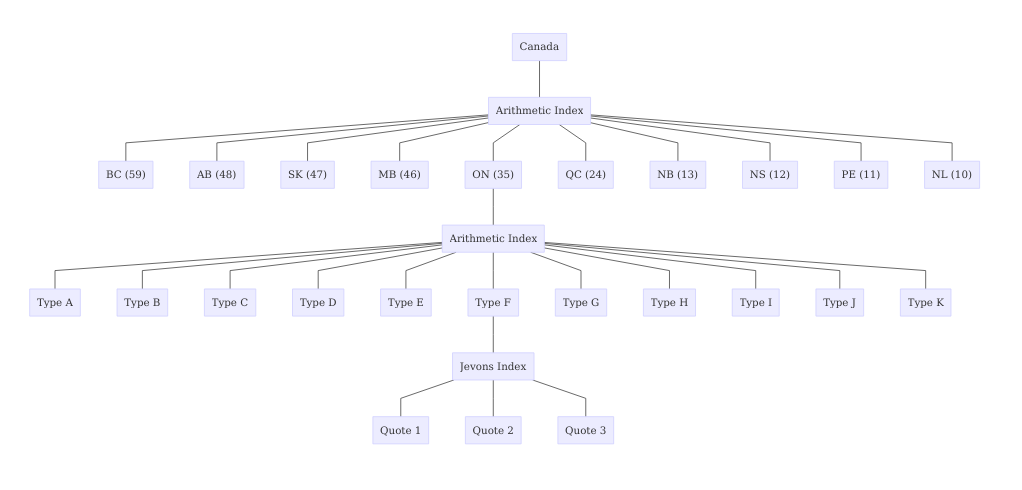
\includegraphics{img/structure.png}

\hypertarget{instructions}{%
\subsection{Instructions}\label{instructions}}

These instructions outline a simple way to build the price index for widgets, although feel free to use a different approach if it's easier. The goal is to understand the process, rather than design the most computationally efficient system. (Hint: look into the dplyr package and the \href{https://github.com/marberts/ppd}{ppd} package for some useful tools.)

Run the following code to grab all the data files and put them in your working environment.

\begin{Shaded}
\begin{Highlighting}[]
\KeywordTok{source}\NormalTok{(}\StringTok{'https://raw.githubusercontent.com/ppd-dpp/price-index-course/master/scripts/get_data.R'}\NormalTok{)}
\end{Highlighting}
\end{Shaded}

\begin{enumerate}
\def\labelenumi{\arabic{enumi}.}
\item
  \textbf{Make the weights}

  Using the \texttt{weights} file, make one set of weights that give the value share of each product sold within each province in each year, and another that gives the value share of all products sold in each province in each year. This first set of weights will be used to aggregate elemental indices to get 10 province-level indices, and the second set of weights will be used to aggregate the province-level indices to a national index. There should be 200 weights in the first file and 20 weights in the second file.
\item
  \textbf{Calculate the geomean for product K}

  Using the microdata for product K in the \texttt{dat\_micro} file, calculate the geometric average of the prices in each province in each month in each reference year. This file should have 250 geomeans.
\item
  \textbf{Calculate the geomean for products A to J}

  Using the data from the Globular Prices System in \texttt{dat\_gps}, calculate the geometric average of the price quotes for each product in each province in each month in each reference year, for products A to J. Combine these data with the data prepared in step 2. The resulting file should have 2,500 geomeans.
\item
  \textbf{Calculate the period-over-period elemental indices}

  For each product in each province in each reference year, calculate the ratio of the geometric averages computed in step 3, making sure to have a price relative of 1 in January 2018 and January 2019. (January 2019 will be the link month when it is time to chain the index.)
\item
  \textbf{Price update the product weights}

  Merge the product-by-province level weights from step 1 into the dataset created in step 4, and use the period-over-period elemental indices to price update the weights.
\item
  \textbf{Calculate the province-level index}

  Calculate an arithmetic index for each province in each reference year, using the period-over-period elemental indices and the price updated weights from steps 4 and 5.
\item
  \textbf{Calculate the Canada-level index}

  Merge the province-level weights in step 1 with the provincial indices from step 6 to calculate a Canada-level index for each reference year.
\item
  \textbf{Chain the 2018 and 2019 indices}

  Chain the 2018 and 2019 province-level and Canada-level indices together, using January 2019 as the link month, to get an index from January 2018 to December 2019 with January 2018 as the base period (usually the base period would be a calendar year, but there are only 24 months of data).
\end{enumerate}

The end result should be a file with 11 price indices, one for each province and a national index, from January 2018 to December 2019, with January 2018 as the base period (= 100).

Validating the Canada-level index requires putting the Canadian Regulatory Economic Analysis group's index and Monsterweb's index into a common form.

\begin{enumerate}
\def\labelenumi{\arabic{enumi}.}
\setcounter{enumi}{8}
\item
  \textbf{Quarter the monthly indices}

  Turn the index you just made and the Canadian Regulatory Economic Analysis group's index in \texttt{index\_crea} into a quarterly index, with quarter 1 2019 as the base period, by taking the average of the three index values in each quarter.
\item
  \textbf{Append all three indices together}

  Put the indices in step 9 together in one dataset with Monsterweb's index in \texttt{index\_mw}. They should all be quarterly with quarter 1 2019 as the base period (= 100).
\end{enumerate}

\hypertarget{references}{%
\section*{References}\label{references}}
\addcontentsline{toc}{section}{References}

\hypertarget{refs}{}
\leavevmode\hypertarget{ref-angrist2009}{}%
Angrist, J., and J-S. Pischke. 2009. \emph{Mostly Harmless Econometrics}. Princeton University Press.

\leavevmode\hypertarget{ref-balk1995}{}%
Balk, B. M. 1995. ``Axiomatic Price Index Theory: A Survey.'' \emph{International Statistical Review/Revue Internationale de Statistique} 63 (1): 69--93.

\leavevmode\hypertarget{ref-balk2008}{}%
---------. 2008. \emph{Price and Quantity Index Numbers}. Cambridge University Press.

\leavevmode\hypertarget{ref-balk2001}{}%
Balk, B. M., and W. E. Diewert. 2001. ``A Characterization of the Törnqvist Price Index.'' \emph{Economics Letters} 72 (3): 279--81.

\leavevmode\hypertarget{ref-bullen2003}{}%
Bullen, P. S. 2003. \emph{Handbook of Means and Their Inequalities}. Springer.

\leavevmode\hypertarget{ref-hausman2003}{}%
Hausman, J. 2003. ``Sources of Bias and Solutions to Bias in the Consumer Price Index.'' \emph{Journal of Economic Perspectives} 17 (1): 23--44.

\leavevmode\hypertarget{ref-cpimanual}{}%
ILO, IMF, OECD, Eurostat, UN, and World Bank. 2004a. \emph{Consumer Price Index Manual: Theory and Practice}. International Monetary Fund.

\leavevmode\hypertarget{ref-ppimanual}{}%
---------. 2004b. \emph{Producer Price Index Manual: Theory and Practice}. International Monetary Fund.

\leavevmode\hypertarget{ref-rppihandbook}{}%
---------. 2013. \emph{Handbook on Residential Property Prices Indices (RPPIs)}. Eurostat.

\leavevmode\hypertarget{ref-kennedy2003}{}%
Kennedy, P. 2003. \emph{A Guide to Econometrics}. 5th ed. MIT University Press.

\leavevmode\hypertarget{ref-kirbymcgregor2019}{}%
Kirby-McGregor, M., and S. Martin. 2019. ``An R Package for Calculating Repeat-Sale Price Indices.'' \emph{Romanian Statistical Review}, no. 3: 17--33.

\leavevmode\hypertarget{ref-kirman1992}{}%
Kirman, A. P. 1992. ``Whom or What Does the Representative Individual Represent?'' \emph{Journal of Economic Perspectives} 6 (2): 117--36.

\leavevmode\hypertarget{ref-lee2016}{}%
Lee, M-J. 2016. \emph{Matching, Regression Discontinuity, Difference in Differences, and Beyond}. Oxford University Press.

\leavevmode\hypertarget{ref-lehmann1998}{}%
Lehmann, E. L., and G. Casella. 1998. \emph{Theory of Point Estimation}. 2nd ed. Springer.

\leavevmode\hypertarget{ref-lord2002}{}%
Lord, N. 2002. ``Does Smaller Spread Always Mean Larger Product?'' \emph{The Mathematical Gazette} 86 (506): 273--74.

\leavevmode\hypertarget{ref-manski1988}{}%
Manski, C. F. 1988. \emph{Analog Estimation Methods in Econometrics}. Chapman Hall.

\leavevmode\hypertarget{ref-manski2007}{}%
---------. 2007. \emph{Identification for Prediction and Decision}. Harvard University Press.

\leavevmode\hypertarget{ref-martin2019}{}%
Martin, S. 2019. ``Moral Management in Competitive Markets.'' \emph{Journal of Economics \& Management Strategy} 28 (3): 541--60.

\leavevmode\hypertarget{ref-mcfadden1978}{}%
McFadden, D. 1978. ``Cost, Revenue, and Profit Functions.'' In \emph{Production Economics: A Dual Approach to Theory and Applications}, edited by M. Fuss and D. McFadden. North-Holland.

\leavevmode\hypertarget{ref-pollak1980}{}%
Pollak, R. A. 1980. ``Group Cost-of-Living Indexes.'' \emph{The American Economic Review} 70 (2): 273--78.

\leavevmode\hypertarget{ref-rosen1974}{}%
Rosen, S. 1974. ``Hedonic Prices and Implicit Markets: Product Differentiation in Pure Competition.'' \emph{Journal of Political Economy} 82 (1): 34--55.

\leavevmode\hypertarget{ref-wooldridge2010}{}%
Wooldridge, J. M. 2010. \emph{Econometric Analysis of Cross Section and Panel Data}. MIT University Press.

\end{document}
